\documentclass[11pt,preprint]{aastex}
% \documentclass[useAMS,usenatbib]{mn2e}
\usepackage{hyperref}
\usepackage{booktabs}
\usepackage{tablefootnote}
\usepackage{amsmath}
\usepackage{breqn}
\usepackage{cite,natbib}
\usepackage{verbatim}
\usepackage{epsfig}
\usepackage{cases}
\usepackage[section]{placeins}
\usepackage{graphicx, subfigure}
\usepackage{color}
\usepackage{amsmath}
\usepackage{float}
\floatplacement{figure}{H}

% \citep[text before][text after]{cite1, cite2}

\newcommand{\logg}{log \emph{g}}
\newcommand{\teff}{$T_{\rm{eff}}$}
\newcommand{\prot}{$P_{rot}~$}

\newcommand{\w}{\mathbf{w}}
\newcommand{\wh}{$\hat{\mathbf{w}}_n$}
\newcommand{\ah}{$\hat{A}_n$}
\newcommand{\ph}{$\hat{P}_n$}
\newcommand{\ch}{$\hat{C}_n$}
\newcommand{\gh}{$\hat{G}_n$}
\newcommand{\yh}{$\hat{Y}_n$}
\newcommand{\teffh}{$\hat{T}_n$}
\newcommand{\chit}{$\chi^2$}

\newcommand{\feh}{[Fe/H]}
\newcommand{\dd}{\ensuremath{\,\mathrm{d}}}

% numbers
\newcommand{\nastero}{310}
\newcommand{\nprecise}{14~}
\newcommand{\ncluster}{211~}
\newcommand{\nHC}{50~}
% \newcommand{\ntotal}{521~}
\newcommand{\ntotal}{365~}
\newcommand{\ngarcia}{310~}
\newcommand{\ncooldwarfs}{45~}
\newcommand{\subcut}{4.1~}

% results
\newcommand{\gyroa}{0.34}
\newcommand{\aerrp}{0.03}
\newcommand{\aerrm}{0.03}
\newcommand{\gyron}{0.58}
\newcommand{\nerrp}{0.02}
\newcommand{\nerrm}{0.01}
\newcommand{\gyrob}{0.34}
\newcommand{\berrp}{0.04}
\newcommand{\berrm}{0.02}
% 3.345395922660827637e-01 3.447082638740539551e-02 3.368341922760009766e-02
% 5.807839035987854004e-01 1.939980983734135300e-02 1.445889472961425781e-02
% 3.414649069309234619e-01 4.333373904228210449e-02 1.554790139198303223e-02

\newcommand{\U}{8}  % mix std
\newcommand{\V}{2.2}  % hot std
\newcommand{\W}{11.4}  % sub std
\newcommand{\X}{14} % mix mu
\newcommand{\Y}{5.0}  % hot mu
\newcommand{\Z}{16.7}  % sub mu
\newcommand{\Q}{0.11}
\newcommand{\Uerrp}{5}
\newcommand{\Uerrm}{3}
\newcommand{\Verrp}{0.7}
\newcommand{\Verrm}{0.6}
\newcommand{\Werrp}{0.6}
\newcommand{\Werrm}{0.5}
\newcommand{\Xerrp}{5}
\newcommand{\Xerrm}{4}
\newcommand{\Yerrp}{0.9}
\newcommand{\Yerrm}{0.8}
\newcommand{\Zerrp}{1.0}
\newcommand{\Zerrm}{0.9}
\newcommand{\Qerrp}{0.07}
\newcommand{\Qerrm}{0.05}
% 5.027511596679687500e+00 8.713015365600584872e-01 7.579417228698730469e-01  % Y hot
% 2.180496454238891602e+00 7.359344959259033203e-01 5.628101825714111328e-01  % V hot
% 1.673530578613281250e+01 9.636192321777343750e-01 9.280376434326171875e-01  % Z sub
% 1.142548561096191406e+01 5.774354934692382812e-01 5.075562667846682530e-01  % W sub
% 1.353189229965209961e+01 4.791536808013916016e+00 4.006250858306884766e+00  % X mix
% 8.121859550476074219e+00 5.122209548950195312e+00 2.673474311828613281e+00  % U mix
% 1.136524602770805359e-01 7.032055407762527466e-02 5.116277188062667847e-02  % P

\begin{document}

\title{Calibrating Gyrochronology using Kepler Asteroseismic targets}

\author{Ruth Angus$^1$, Suzanne Aigrain$^1$,
Daniel Foreman-Mackey$^2$, Amy McQuillan$^3$}
\affil{$^1$Department of Physics, University of Oxford, OX1 3RH, UK}
\affil{$^2$Centre for Cosmology and Particle Physics, New York University, New
York, NY, USA}
\affil{$^3$School of Physics and Astronomy, Raymond and Beverly Sackler,
Faculty of Exact Sciences, Tel Aviv University, 69978, Tel Aviv, Israel}

\begin{abstract}
\label{abs}

Among the available methods for dating stars, gyrochronology is a powerful one
because it requires knowledge of only the star's mass and rotation period.
However, it is not well calibrated at late ages and suffers from large
systematic uncertainties.
Asteroseismology provides age measurements for some of the brightest stars
observed by {\it Kepler}.
We use rotation period measurements of \nastero$~$stars with asteroseismic
ages, \nHC stars from the Hyades and Coma Berenices clusters and 5 field stars
(including the Sun) with precise age measurements to calibrate the
gyrochronology relations.
We model the relationship between rotation period, age and colour while
accounting for measurement uncertainties in all three quantities.
Our sample includes both MS stars and subgiants, and straddles the Kraft break.
Only MS stars cooler than the Kraft break, at approximately 6250 K, are
expected to follow gyrochronology relations; this must be taken into account
when modelling the data.
In principle, our method enables us to estimate an age for any cool MS star
with a measured rotation period and colour, along with an associated
uncertainty that reflects both measurement errors and the intrinsic scatter in
the gyrochronology relations.
Such an approach is adjustable for any gyrochronology study.
We used Markov chain Monte Carlo (MCMC) to explore posterior probability
distribution functions of the gyrochronology parameters and carefully checked
the effects of leaving out parts of our sample, leading us to find that no
single relation beween rotation period, colour and age can adequately describe
all the clusters used in this analysis.
This may have concerning consequences for the overall reliability of
gyrochronology as a dating method---further investigation into the level of
intrinsic scatter in the gyrochronology parameters will be required.

\end{abstract}

\section{Introduction}
\label{intro}
\subsection{Dating methods for field stars}

Many fields of astronomy rely on precise age measurements of Main Sequence
(MS) stars.
Unfortunately, age is a notoriously difficult quantity to measure for these
stars, as observable properties evolve slowly on the MS.
Even with high precision spectroscopic measurements, ages often cannot be
determined accurately to within 20\% \citep{Soderblom2010}.
Some of the most precise age measurements currently available are for stars in
clusters where isochrones can be fitted to a coeval population with a range of
masses, resulting in age measurements with uncertainties often as low as 10\%.
Isochronally derived {\it field} star ages, on the other hand, are much less
precise than this, often having uncertainties of around 50\% or more.
Demand for age estimates of planet-hosting stars is high, but faint stars
observed by {\it Kepler} are often expensive or impractical spectroscopic
targets.
Where high resolution spectra are unavailable, gyrochronology can be
extrememly useful.
Gyrochronology is a dating method that utilises the predictable rotation
period evolution of low mass, MS stars.
It requires only knowledge of the rotation period---which is often easily
extracted from {\it Kepler} light curves---and mass (or appropriate proxy) of
a star.
However the current gyrochronology relations are entirely empirically
calibrated and still need refining at large stellar ages.
{\it Kepler} provides the perfect opportunity to calibrate gyrochronology at
late ages---it provides surface rotation periods of thousands of stars and new
age estimates for hundreds of stars via asteroseismology.
This paper aims to use these new asteroseismic age measurements to improve the
gyrochronology relations at late ages.

\subsection{Gyrochronology}

Mass loss via a magnetised stellar wind causes magnetic braking of MS stars
\citep{Weber1967}.
A dynamo-driven magnetic field, generated at the tachocline (the interface
between radiative and convective zones) locks the stellar wind to the surface
of the star.
The stellar wind corotates with the stellar surface out to the Alfv\'{e}n
radius, at which point it decouples and angular momentum is lost from the
star.
The strength of the magnetic field at the surface, and therefore the rate of
angular momentum loss, is related to rotation period \citep{Kawaler1988}.
Due to this dependence, although stellar populations are born with a range of
rotation periods, the rapid rotators rapidly lose angular momentum and
rotation periods converge onto a well-defined sequence.
The timescale for convergence is around the age of the Hyades for solar mass
stars: 650 Myrs \citep{Radick1987, Irwin2009}.
After this time, rotation periods are \emph{independent} of their initial
values.
Gyrochronology postulates that each star falls on a single three-dimensional
plane described by mass, rotation period and age, i.e. given any two of these
three properties, one can determine the third.
The form of angular momentum evolution described above and calibrated in this
article can only be applied to F, S and K MS stars.
Fully convective M dwarfs have a different dynamo-driven magnetic field: their
rotation periods evolve over extremely long timescales and they often do not
converge onto the mass-period-age plane, even after several Gyrs.
Hot stars with effective temperatures $\gtrsim$ 6250 K have shallow convective
zones---they are almost fully radiative---and, again, they have a different
dynamo-driven magnetic field \citep{Kraft1967}.
These massive stars retain their initial rotation period throughout their
brief MS lifetimes and are therefore not suitable gyrochronology targets.

The rate of rotation period decay for intermediate mass MS stars was first
quantified by \citet{Skumanich1972}, who observed that rotation period,
lithium abundance and chromospheric activity decay was proportional to the
square-root of age.
Later, \citet{Noyes1984_2} added a mass dependence to the period-activity-age
relation after more massive stars were observed to spin down more slowly.
The term `gyrochronology' was coined by \citet{Barnes2003} who proposed an
empirically motivated functional form for the relation between period, colour
and age, \begin{equation} \label{eq:Barnes2007_2} P = A^n \times a(B-V-c)^b,
\end{equation} where $P$ is rotation period (in days), $A$ is age (in Myr),
$B$ and $V$ are B and V band magnitudes respectively and $a$, $b$, $c$ and $n$
are constants.

This gyrochronology relation was calibrated using open clusters, which are
invaluable calibration tools since their ages are known relatively precisely
and each cluster contains many stars of the same age which enables the
period-mass relation to be tightly constrained.
Unfortunately however, the majority of nearby clusters are young and until
recently it was difficult to measure rotation periods for all but the
youngest, most active stars (using ground--based observations).
There is a significant dearth of precisely measured ages for old stars and it
is for this reason that the current gyrochronology relations are poorly
calibrated at late ages.
\citet{Barnes2007} used 8 young open clusters aged between 30 and 650 Myrs to
calibrate the dependence of rotation period on mass, and the Sun to calibrate
the dependence on age.
Best-fit values of $n$, $a$ and $b$ ($c$ was fixed at 0.4) reported in
\citet{Barnes2007} are presented in table \ref{tab:constants}.
Equation \ref{eq:Barnes2007_2} was further calibrated by \citet{Mamajek2008}
using updated rotation period and age measurements of stars in open clusters
$\alpha$ Per \citep{Prosser1995}, Pleiades \citep{Prosser1995,
Krishnamurthi1998}, M34 \citep{Meibom2011_M34}, and Hyades \citep[Henry,
private comm.,][]{Radick1987, Radick1995, Prosser1995, Paulson2004}.
Once again, the Sun was used as an age anchor---a single data point specifying
the shape of the period-age relation.
Whereas \citet{Barnes2007} fixed the position of $c$, the `colour
discontinuity' in equation \ref{eq:Barnes2007_2}, at 0.4, \citet{Mamajek2008}
allow it to be a free parameter in their model.
The values of $n$, $a$ and $b$, resulting from their fit are shown in table
\ref{tab:constants}.
In both of these studies a maximum likelihood fitting approach was used.
This method relies on the assumption that uncertainties are Gaussian, which
may not always be the case, and only takes observational uncertainties on the
dependent variable into account.
As described in \textsection \ref{sec:gyro_cal}, we adopt a fitting method
that properly accounts for uncertainties on all three observed variables:
colour, period and age.

\begin{deluxetable}{lccc}
\tablewidth{0pc}
\tablecaption{Values of a, b, c and n in \citet{Barnes2007} and
	\citet{Mamajek2008} and Angus et al. (2014).
\label{tab:constants}}
\tablehead{
\colhead{Parameter}&
\colhead{\citet{Barnes2007}}&
\colhead{\citet{Mamajek2008}}&
\colhead{Angus et al. (2014)}}
\startdata
a & $0.7725 \pm 0.011$ & $0.407 \pm 0.021$ & $\gyroa^{+\aerrp}_{-\aerrm}$ \\
b & $0.601 \pm 0.024$ & $0.325 \pm 0.024$ & $\gyrob^{+\aerrp}_{-\berrm}$\\
c & $0.4$ & $0.495 \pm 0.010$ & $0.45$ \\
n & $0.5189 \pm 0.0070$ & $0.566 \pm 0.008$ & $\gyron^{+\nerrp}_{-\nerrm}$\\
\enddata
\end{deluxetable}

The data used in this article are described in \textsection \ref{sec:data},
our calibration and model fitting process is outlined in \textsection
\ref{sec:gyro_cal} and the results are presented and discussed in \textsection
\ref{sec:results}.

\section{Observations}
\label{sec:data}

The ages of 505 {\it Kepler} dwarfs and subgiants were published by
\citet{Chaplin2014}.
They made use of two global asteroseismic parameters---the average large
frequency separation and the frequency of maximum oscillations power---to
estimate stellar properties, including the ages, with a grid-based approach
that utilised several different search codes coupled to more than ten grids of
stellar evolutionary models.

The ages quoted in \citet{Chaplin2014} come from one of the grid-code
combinations, with uncertainties reflecting the scatter between the different
sets of results.
\citet{Chaplin2014} used two different sets of effective temperatures: one was
derived using an Infra-Red Flux Method (IRFM) calibration
\citep{Casagrande2010, SilvaAguirre2012} and the other from a recalibration of
the SDSS griz filter KIC photometry by \citet{Pinsonneault2012} using Yale
Rotating Stellar Evolution Code (YREC) models \citep{Demarque2004}.
We use the IRFM temperatures since they are less dependent on metallicity,
which is not well constrained for the asteroseismic sample, and their
uncertainites are more conservative, however our analysis is relatively
insensitive to this choice.
87 stars in the asteroseismic catalogue have spectroscopic measurements of
\teff$~$, and [Fe/H].
These precisely measured spectroscopic properties allowed more tightly
constrained ages to be calculated for these 87 stars, which were
incorporated where available.
In order to produce a relation that predicts the age of a star using only
observable properties, we chose to convert \teff$~$to $B-V$ for the
asteroseismic sample using the relation of \citet{Sekiguchi2000}.
This conversion added an extra element of noise to our data since the
metallicities provided for the asteroseismic stars are simply an average value
for the field: $-0.2\pm0.3$ dex \citep[see e.g.][]{Silva_Aguirre2011}.
However, since the age uncertainties dominate this analysis, we do not expect
this to have a significant impact on our results.

The ages quoted in Chaplin et al. (2014) have typical uncertainties of 35\%.
These large uncertainties are the result of the fact that only approximate
inferences can be made on the ages using the global asteroseismic parameters,
neither of which has an explicit dependence on age.
It will be possible, however, to derive more precise ages for a subset of
these stars.
By measuring the frequency of each oscillation mode individually,
not just the global asteroseismic parameters, one can provide much tighter
constraints on ages.
% not just the
% mean large separation, one can build up a density profile of the star and
% provide a tighter constraint on its age.
Ages derived from individual oscillation mode measurements can have
uncertainties as small as 10\% \citep{Brown1994, SilvaAguirre2013}.
However, measuring frequencies for individual oscillation modes is a manual
process and can only be applied in the highest signal-to-noise cases.
\citet{Chaplin2014} predict that around 150 of the 505 stars will be suitable
for this individual oscillation mode treatment.
We obtained precise ages for 42 stars from \citet{Metcalfe2014}, modelled with
the Asteroseismic Modeling Portal (AMP), with effective temperatures and
metallicities from \citet{Bruntt2012}.
Of the 42 stars in \citet{Metcalfe2014}, we only incorporate the `simple
stars' (cool dwarfs) into our sample, ignoring the hotter F stars and more
evolved subgiant stars as these are not expected to follow the simple
gyrochronology relation.
% It should be noted that, due to a technical issue with their stellar evolution
% code, ages for stars with small convective cores were incorrectly estimated in
% \citet{Chaplin2014}.
% This issue is acknowledged in \citet{Metcalfe2014} and should not affect our
% analysis since it concerns stars that are hotter than the Kraft break and
% therefore not expected to follow the gyrochronology relation.

The {\it Kepler} light curves of the 505 asteroseismic targets display
quasi-periodic variations on timescales corresponding to the rotational
periods of the stars---flux variations are produced by active regions on the
stellar surface that rotate in and out of view.
Rotation periods for \ngarcia of these stars are published in
\citet{Garcia2014} who used a combination of an autocorrelation function and
wavelet transform method to measure surface rotation.
From the 505 targets in the original sample, \nastero$~$rotation periods were
reliably measured, \nprecise of which have precise asteroseismic ages from AMP
modelling.
All stars in the asteroseismic sample with rotation periods published by
\citet{McQuillan_2014}, also appear in the rotation period catalogue of
\citet{Garcia2014}.
There is excellent agreement between rotation period
measurements where the two catalogues overlap.

The asteroseismic sample covers a large range of ages, however it does not
provide good mass coverage across the entire range (see figures
\ref{fig:p_vs_a} and \ref{fig:3d}).
Few stars have temperatures below 6000 K ($B-V$ $\sim$ 0.55) and of the low
mass stars, most of them are old (note that massive stars evolve rapidly and
so we do not expect many in the sample).
We therefore added \nHC stars to our sample from young clusters Coma Berenices
(0.5 Gyr), and the Hyades (0.625 Gyr) (see table \ref{tab:clust}).
Clusters younger than 0.5 Gyr often have large populations of rapid rotators
that have not yet converged onto the gyrochronology plane, so no clusters
younger than Coma Ber were included.
Uncertainties on $B-V$ colours associated with each cluster star were not
provided in the catalogues from which rotation periods and ages were obtained.
Since the uncertainty associated with each measurement plays such a key role
in our analysis (see \textsection \ref{sec:gyro_cal}), we assigned an
uncertainity of $\pm 0.04$ mag to each colour measurement, based on the mean
uncertainty in the asteroseismic temperature-converted colours.
The 1.1 and 0.588 Gyr open clusters, NGC 6811 and Praesepe, were originally
included in our analysis.
However we discovered that their period-colour relations were different to
those of the Hyades and Coma Ber, as well as to each other's, and we therefore
did not include them in our final analysis.
A further 5 field stars with precise age measurements were added to the
sample: 16 Cyg B, Alpha Cen A and B, 18 Sco and, of course, the Sun (see table
\ref{tab:field}).
The entire set of \ntotal stars is shown in figures \ref{fig:p_vs_a} and
\ref{fig:3d}.
Asteroseismic targets are shown in black, with cluster and field stars in blue
and the Sun in red.
\begin{deluxetable}{lcccc}
\tablewidth{0pc}
\tablecaption{Clusters and References: (1) \citet{Dobbie2009},
	(2) \citet{CollierCameron2009}, (3) \citet{Perryman1998},
	(4) \citet{Radick1987}.}
\label{tab:clust}
\tablehead{
\colhead{Cluster}&
\colhead{Age (Gyr)}&
\colhead{Number of stars}&
\colhead{Age ref}&
\colhead{Rotation period ref}}
\startdata
Coma Ber & 0.5 $\pm$ 0.1 & 28 & 1 & 2 \\
Hyades & 0.625 $\pm$ 0.05 & 22 & 3 & 4 \\
\enddata
\end{deluxetable}

\begin{deluxetable}{lccc}
\tablewidth{0pc}
\tablecaption{Rotation periods and $B-V$ colours for field stars with precise
	ages. References: (a) \citet{Metcalfe2012}, (b) \citet{Davies2014}, (c)
\citet{Moffett1979}, (d) \citet{Li2012}, (e) \citet{Petit2008}, (f)
\citet{Mermilliod1986}, (g) \citet{Bouvier2010}, (h) \citet{Donahue1996}, (i)
\citet{Cox2000}, (j) \citet{Bazot2012}, (k) \citet{Yildiz2007}, (l)
\citet{Hallam1991}, (m) \citet{Dumusque2012}.
Notes: \citet{Davies2014} measured an internal rotation period for 16 Cyg B
using asteroseismology.
However, this is likely to be close to the surface rotation value.
Rotation periods for and $\alpha$ Cen A and B were measured
from variation in chromospheric emission lines.
High-resolution spectropolarimetric observations were used to measure
a rotation period for 18 Sco.
The age of 16 Cyg B was measured with asteroseismology.
18 Sco's age measurement was based chiefly on an asteroseismic analysis,
however its rotation period was used as an additional constraint, so the age
estimate is not entirely independent of rotation period for this star.
An age for the $\alpha$ Cen system was estimated from spectroscopic
observations with additional seismic constraints.}
\label{tab:field}
\tablehead{
\colhead{ID}&
\colhead{age}&
\colhead{\prot}&
\colhead{$B-V$}}
\startdata
16 Cyg B & 6.4 $\pm$ 0.4$^a$ & 23.2 $^{+11.5}_{-3.2}$$^b$ & 0.66 $\pm$ 0.01$^c$ \\
18 Sco & 3.7 $\pm$ 0.2$^d$ & 22.7 $\pm$ 0.5$^e$ & 0.64 $\pm$ 0.01$^f$ \\
The Sun & 4.568 $\pm$ 0.001$^g$ & 26.09 $\pm$ 0.1$^h$ & 0.65 $\pm$ 0.001$^i$ \\
$\alpha$ Cen A & 6 $\pm$ 1$^{j, k}$ & 28.8 $\pm$ 2.5$^{l}$ &
0.69 $\pm$ 0.01$^f$ \\
$\alpha$ Cen B & 6 $\pm$ 1$^{j, k}$ & 38.7 $\pm$ 5.0$^{m}$ &
0.90 $\pm$ 0.01$^f$ \\
\enddata
\end{deluxetable}

\section{Calibrating the Gyrochronology relation}
\label{sec:gyro_cal}

\subsection{The model}

The \nastero$~$asteroseismic stars in our sample have $B-V$ colours converted
from effective temperatures, photometric rotation periods,
asteroseismic ages, and asteroseismic surface gravities.
Each measurement of these properties is assumed to be independent with an
associated Gaussian uncertainty.
Not all of the cluster stars added to our sample have \logg$~$values; however,
since we only use \logg$~$to separate the populations of subgiants and dwarfs
(and we assume that the cluster stars are dwarfs) this should not affect our
results.
Following the treatment of \citet{Barnes2007} and \citet{Mamajek2008},
rotation period was treated as the dependent variable throughout the modelling
process.

Hot stars and subgiants follow a different gyrochronology relation to MS
dwarfs.
Stars with effective temperatures above the Kraft-break, $T_{\rm{eff}}
\sim$ 6250 K, \citep{Kraft1967} do not have a thick convective envelope and
cannot support a strong magnetic dynamo, so do not spin down appreciably
during their MS lifetimes.
Subgiants spin down rapidly as they expand due to angular momentum
conservation and thus diverge from the gyrochronological mass-period-age
plane.
The point in their evolution at which they depart, the `gyrochronological MS
turn off', is difficult to define.
Classically, MS turnoff is defined as the hottest point on a star's path on
the HR diagram (before it ascends the giant branch) but theory predicts that
evolving stars begin the process of spinning down relatively slowly after
leaving the classically defined MS \citep{vanSaders2013}.
For this reason we chose a very simple definition of MS turnoff: we defined
a \logg$~$boundary of \subcut to mark the transition between dwarfs and
giants.
We trialed a range of boundary values and found that \subcut minimised subgiant
contamination whilst maximising the cool dwarf sample.
It was also necessary to use a mixture model to account for misclassified
subgiants---without it, subgiant contamination significantly biased the
resulting fit.
We did not exclude hot stars and subgiants from our sample during the
modelling process, we modelled all three populations simultaneously.
This allowed for the fact that stars have some probability mass lying in all
three regimes due to their large observational uncertainties.
% In addition to hot stars and subgiants, there was a further population of
% contaminating stars in our sample: rapid rotators.
% These stars do not lie on the standard gyrochronology mass-period-age plane
% and could plausibly be synchronised binaries, stars with unseen, close-in,
% massive planets \citep{Poppenhaeger2014, Beky2014} or stars which have not
% yet converged onto the gyrochronology plane.

Hot MS stars were defined as those with $B-V$ $<$ 0.45, corresponding to
\teff$~\approx$ 6250 K for solar metallicity and \logg.
Since there is no dependence of rotation period on age for massive MS stars,
their rotation periods were modelled as a normal distribution with mean and
standard deviation, $Y$ and $V$, as free parameters.
Subgiant rotation periods \emph{do} depend on age and $T_{\rm{eff}}$.
However, since the rotational properties of these stars are not interesting for
the purposes of gyrochronology calibration, we also modelled them with
a normal distribution with mean and standard deviation, $Z$ and $U$, as free
parameters.
We used a mixture model for the remaining population of stars, consisting of
cool dwarfs and misclassified, contaminating subgiants.
The subgiants were treated as if their rotation periods had been drawn from
a background normal distribution with mean and standard deviation, $X$ and
$U$, again inferred from the data and another parameter, $Q$, the
probability of each star belonging to that background population.
The results of this analysis were not particularly sensitive to the choice of
distribution for the hot stars and subgiants.
These models were put in place so that we did not have to throw any data
away and we could model everything at once.
% This was important due to the large uncertainties on the observational
% parameters.
This was important because stars were classified according to their observed
temperatures and \logg s, which are noisy.
Due to the large uncertainties on \teff$~$and \logg, each star therefore has some
probability of being a subgiant, some of being a cool dwarf and some of
being a hot star.
By throwing away data, one could accidentally throw away a misclassified star.
We avoid this problem by modelling all stars simultaneously and taking a
probabilistic approach to classification.
Inferences made about the parameters of the normal distributions used to model
subgiants and hot stars were not of particular interest for the purposes of
gyrochronology calibration.
We decided to use simple normal distributions rather than more physically
motivated models in order to remain as model--independent as
possible.
% We chose to use a Gaussian distribution because it is the maximum entropy
% distribution, and therefore the most conservative choice, with only two
% parameters.

% The boundaries separating cool dwarfs, hot dwarfs and subgiants left only
% \ncooldwarfs stars classified as cool dwarfs (plus some contaminating
% subgiants) in our asteroseismic sample, 6 of which have precise ages from AMP
% modelling (see figure \ref{fig:logg_vs_t}).
% These boundaries were placed in order to avoid {\it all} potential
% contamination from subgiants which rotate more slowly than MS stars and, if
% left in the sample, would have significantly biased the resulting
% gyrochronology relation.
Ideally both the hot star ($B-V$ $<$ 0.45) and subgiant (\logg$~<$\subcut)
boundaries would be free parameters in our model.
However, since these two populations were modelled with a relatively
unconstraining normal distributions, these boundary parameters would not be
well behaved.
Both would be pushed to higher and higher values until all stars were modelled
with a normal distribution.
In order to avoid this problem, we fixed these two boundaries.
A future analysis could avoid the assumption that the gyrochronology relation
is infinitely narrow and assign it some intrinsic width, which would also be
a free parameter.

We postulate that there is a deterministic relationship between the `true'
rotation period of a cool MS star and its `true' age and colour, described by
equation \ref{eq:Barnes2007_2} (by `true' we mean the value an observable
property would take, given extremely high signal-to-noise measurements).
Rotation period also depends on \logg$~$since this property determines whether
a star falls in the dwarf or subgiant regime.

In what follows we use $P$ to denote rotation period and define
$\mathbf{w} = (age, B-V,~\log~g)$ as the vector of additional observational
properties.
Observations are denoted as \ph$~$and $\hat{\mathbf{w}}_n$ and the unobserved
(latent), `true' parameters as $P_n$ and $\mathbf{w}_n$ for stars $1,...,N$.

In order to explore the posterior Probability Distribution Functions (PDFs) of
the model parameters, $\theta$, conditioned on a set of noisy observations,
$\{\hat{P}_n, \hat{\mathbf{w}}_n\}$, it was necessary to marginalise over the
latent parameters, $\{P_n, \mathbf{w}_n\}$.
Assuming all measurements are independent, the marginalised likelihood can be
written
\begin{equation}
	p(\{\hat{P}_n,\hat{\w}_n\}|\theta) =
	\prod_{n=1}^{N} \int p(\hat{P}_n,\hat{\w}_n,P_n,\w_n|\theta)
	{\rm d}P_n {\rm d}\w_n.
\label{eq:fulll}
\end{equation}
The joint probability, on the right hand side of this equation, can be
factorised as
\begin{align}
	p(\hat{P}_n,\hat{\w}_n,P_n,\w_n|\theta) = p(P_n\,| & \,\w_n,\theta)
	p(\hat{P}_n\,|\,P_n)\,p(\hat{\w}_n\,|\,\w_n)p(\w_n),
\nonumber
\end{align}
where we have utilised the fact that the observations, \ph$~$and \wh$~$are
{\it conditionally independent} of the model parameters, $\theta$: they only
depend on $\theta$ through the latent parameters, $P_n$ and $\w_n$.
The above integral can  be written
\begin{equation}
	p(\{\hat{P}_n,\hat{\w}_n\}|\theta) \propto
	\prod_{n=1}^{N} \int p(\w_n|\hat{\w}_n)
	{\rm d}\w_n \int p(P_n|\w_n,\theta) p(\hat{P}_n\,|\,P_n) {\rm d}P_n,
\label{eq:fac}
\end{equation}
where we have used Bayes' theorem:
$p(\w_n|\hat{\w}_n) \propto p(\hat{\w}_n|\w_n)p(\w_n)$.
The outer integral is the same for hot dwarfs, cool dwarfs and subgiants
alike.
In our model, the probability of the `true' rotation period given the `true'
observed parameters and the model parameters, $p(P_n|\w_n, \theta)$, is
different in each regime because a different generative process is responsible
for producing rotation periods.
For cool dwarfs ($B-V$ $<$ 0.45 and \logg$~>$ \subcut):
\begin{eqnarray}
	p(P_n|\w_n,\theta) =
	& (1-Q)~\delta \left (P_n - \left[A^n \times a(B-V - c)^b\right]
	\right) \quad \\ & +~Q~\left(\sqrt{2\pi U^2}\right)^{-1/2}
	~\exp\left({-\frac{(P_n-X)^2}{2U^2}}\right),
\end{eqnarray}
where $Q$ is the probability that a star is drawn from the population of
misclassified subgiants.
For hot dwarfs ($B-V$ $<$ 0.45 and \logg$~>$ \subcut) the generative process
is:
\begin{eqnarray}
p(P_n\,|\,\w_n,\theta) = \left(\sqrt{2\pi V^2}\right)^{-1/2}~
\exp\left({-\frac{(P_n-Y)^2}{2V^2}}\right),
\end{eqnarray}
and for subgiants,
\begin{eqnarray}
p(P_n\,|\,\w_n,\theta) = \left(\sqrt{2\pi W^2}\right)^{-1/2}~
\exp\left({-\frac{(P_n-Z)^2}{2W^2}}\right).
\end{eqnarray}

We used hierarchical inference to account for observational uncertainties,
following the method of \citet{Hogg2010}, also used by
\citet{Foreman-Mackey2014}, \citet{Rogers2014}, \citet{Morton2014} and
\citet{Demory2014}.
We computed equation \ref{eq:fac} up to an unimportant constant
using a sampling approximation.
The values of \ph$~$and \wh$~$with uncertainties, $\sigma_P$ and
$\sigma_{\mathbf{w}}$, reported in catalogues provide constraints on the
posterior probability of those variables, under a choice of prior PDF,
$p_0(\hat{\mathbf{w}}_n)$.
Ideally, these catalogues would provide posterior PDF samples, not just point
estimates, which we could use directly.
i.e. samples from
\begin{equation}
% 	p(\hat{\mathbf{w}}_n|D_n) =
% 	\frac{p(D_n|\hat{\mathbf{w}}_n)p_0(\hat{\mathbf{w}}_n)}
% 	{p_0(D_n)},
	p(\mathbf{w}_n|\hat{\mathbf{D}}_n) =
	\frac{p(\hat{\mathbf{D}}_n|\mathbf{w}_n)p_0(\mathbf{w}_n)}
	{p_0(\hat{\mathbf{D}}_n)},
\end{equation}
where $p(\hat{\mathbf{D}}_n|\w_n)$ is the likelihood of the data,
$\hat{\mathbf{D}}_n$ (in this case,
the set of {\it Kepler} lightcurves plus spectroscopic \teff$~$and
\feh$~$measurements), given the model parameters, $\mathbf{w}_n$.
$p_0(\hat{\w}_n)$ is an uninformative prior probability distribution
function $p_0(\mathbf{w}_n)$ is an uninformative prior PDF, chosen by the
fitter \citep[][used a flat prior PDF in age and \logg]{Chaplin2014}.
In the absence of posterior PDF samples\footnote{Posterior PDF samples
for asteroseismic parameters are now beginning to be published and will be made
available in future publications.} we generated our own from Gaussian
distributions with means, \wh$~$and standard deviations, $\sigma_{\mathbf{w}}$.
$J$ posterior samples were generated for each star (we used $J$ = 100):
\begin{eqnarray}
\w_n^{(j)} &\sim& p(\w_n\,|\,\hat{\w}_n),
\end{eqnarray}
and were used to evaluate $p(\mathbf{w}_n|\hat{\mathbf{w}}_n)$ up to a
normalisation constant.
% We then evaluated the marginalized likelihood for a single star as follows
Using these samples we computed the marginalised likelihood for a single
star as follows,
\begin{align}
% 	p(\hat{P}_n,\hat{\w_n}\,|\,\theta) \approx \frac{1}{J_n}
% 	\sum_{j=1}^{J_n}p(\hat{P}_n\,|\,\mathbf{w}_n^{(j)},\theta).
	p(\hat{P}_n,\hat{\w_n}\,|\,\theta) \approx \frac{1}{J_n}
	\sum_{j=1}^{J_n}p(P_n\,|\,\mathbf{w}_n^{(j)},\theta)p(\hat{P}_n|P_n).
\end{align}
% where $P_n^{(j)}$ was computed from the posterior PDF samples.
For the cool dwarfs, $p(P_n|\mathbf{w}_n^{(j)}, \theta)p(\hat{P}_n|P_n)$,
has a $\delta$-function component and a Gaussian component and can
therefore be integrated analytically.
For the subgiants and hot dwarfs,
$p(P_n|\mathbf{w}_n^{(j)}, \theta)p(\hat{P}_n|P_n)$ is the product of two
Gaussians, which is another Gaussian and, again, this integral is analytic.
% For samples falling in the cool dwarf regime, $P_{n,j}$ was computed
% using equation \ref{eq:Barnes2007_2}.
% For those samples falling in the hot dwarf or subgiant regimes, $P_{n,j}$ was
% set equal to the mean of the normal distribution: $Y$ for hot dwarfs; $X$ for
% `misclassified' subgiants with \logg$~>4.1$ and $Z$ for subgiants with
% \logg$~<4.1$.
Finally, the marginalised log-likelihood can be written
\begin{eqnarray}
	\log p(\{\hat{P}_n,\hat{\w}_n\}\,|\,\theta) &\approx&
	\log \mathcal{Z} + \sum_{n=1}^N
	\log \left[ \sum_{j=1}^{J_n}p(P_n\,|\,\mathbf{w}_n^{(j)}, \theta)p(\hat{P}_n|P_n) \right ]
\end{eqnarray}
where $\mathcal{Z}$ is an irrelevant normalisation constant.
We used {\tt emcee} \citep{Foreman-Mackey2013}, an affine invariant, ensemble
sampler Markov Chain Monte Carlo (MCMC) algorithm, to explore the posterior
PDFs of the model parameters, $\theta$.
Flat prior PDFs were used for each parameter.
Following the above method, a likelihood was computed as follows:
\begin{itemize}
	\item For each star, $J$ samples were drawn from three normal
		distributions: one in colour, one in age and one in \logg,
		where the means and standard deviations of those distributions
		were the observed values and uncertainties.
		This step was performed just once and the
		following steps were performed for each likelihood evaluation.
	\item For those samples that fell in the cool dwarf regime
		($B-V$ $>$ 0.45 and \logg$~>$ \subcut), model rotation
		periods were both calculated using equation
		\ref{eq:Barnes2007_2} and assigned the value of parameter $X$.
% 		In the case that the sample was better described by equation
% 		\ref{eq:Barnes2007_2} than by the normal distribution with mean
% 		and standard deviation $X$ and $U$, that sample
		A Likelihood for the two model rotation periods were then
		evaluated using a Gaussian mixture model
		likelihood function.
	\item For the samples that fell in the hot dwarf ($B-V$ $<$ 0.45 and
		\logg$~>$ \subcut) and subgiant (\logg$~<$ \subcut) regimes,
		likelihoods were calculated by comparing observed rotation
		periods with the model rotation periods for the two
		populations: $Y$ and $Z$.
	\item The total log-likelihood for each star was calculated as the
		sum of the log-likelihoods of each of the $J$ samples.
	\item Finally, the sum of individual star log-likelihoods
		provided the total log-likelihood.
\end{itemize}

\section{Results and Discussion}
\label{sec:results}

\begin{deluxetable}{lccc}
\tablewidth{0pc}
\tablecaption{Median values of a, b, c and n for individual clusters.
\label{tab:cluster_results}}
\tablehead{
\colhead{Parameter}&
\colhead{Coma Berenices}&
\colhead{Hyades}}
\startdata
a & $0.417^{+0.08}_{-0.07}$ & $0.312^{+0.04}_{-0.06}$ \\
b & $0.271^{+0.05}_{-0.06}$ & $0.410^{+0.05}_{-0.04}$ \\
n & $0.542 \pm 0.03$ & $0.599^{+0.03}_{-0.02}$ \\
\enddata
\end{deluxetable}

A gyrochronology relation was initially fit to the asteroseismic stars, the
field stars and four clusters (Hyades, Coma Berenices, Praesepe and NGC 6811)
all together.
However, this resulted in extremely multi-modal posteriors PDFs for
$a$, $b$ and $n$ and a best-fitting model which significantly overpredicted
the age of the Sun.
After fitting a separate relation to various subsets of the data, it became
evident that the multi-modal posterior PDF was only produced when Praesepe and
NGC 6811 were included in our sample.
The reason for this multimodality is unclear, however we tentatively attribute
it to the position of the colour discontinuity, $c$ taking a different value
for Praesepe than for the Hyades and Coma Berenices and the shape of the
period-colour relation for NGC 6811 being discrepant.
We calculated the likelihood for Praesepe, plus the field stars (to provide
the age dependence) with two different values of $c$: $0.45$ and $0.5$,
finding a higher likelihood for $c=0.5$.
Since we do not fully understand the cause of this variation in $c$, and in
order to keep our model simple, we chose to exclude Praesepe and NGC 6811 from
our final data set and fit a gyrochronology relation with $c=0.45$ to the
remaining data (asteroseismic stars, field stars, Hyades and Coma Ber).
We also fitted relations with $c$ values ranging from 0.4 to 0.55 to this final
data set, finding that the results were relatively insensitive to variations
in this parameter (solar ages predicted from each best-fitting model were
consistent).
Individual fits to Hyades and Coma Berenices, plus the field stars are shown
in figures \ref{fig:CF45} and \ref{fig:HF45}.
50th percentile parameter values with their 16th and 84th
percentile uncertainties for the two clusters are provided in table
\ref{tab:cluster_results}.
Note that none of these parameters are fully consistent between the two
clusters; there seems to be some intrinsic scatter in the gyrochronology
parameters.
The fact that each cluster seems to prefer a different value of $a$, $b$, $n$
and $c$ paints a concerning picture for gyrochronology which assumes one set
of parameters can be used to describe all stars.
\begin{deluxetable}{lcc}
\tablewidth{0pc}
\tablecaption{Median values of the parameters describing the populations of
	non-gyrochronological stars.
\label{tab:nuisance}}
\tablehead{
\colhead{Parameter}&
\colhead{Median value}}
\startdata
$U$ & \U$^{+\Uerrp}_{-\Uerrm}$ days \\
$V$ & \V$^{+\Verrp}_{-\Verrm}$ days \\
$W$ & \W$^{+\Werrp}_{-\Werrm}$ days \\
$X$ & \X$^{+\Xerrp}_{-\Xerrm}$ days \\
$Y$ & \Y$^{+\Yerrp}_{-\Yerrm}$ days \\
$Z$ & \Z$^{+\Zerrp}_{-\Zerrm}$ days \\
$Q$ & \Q$^{+\Qerrp}_{-\Qerrm}$ \\
\enddata
\end{deluxetable}

The fits to the final data set are shown in figures
\ref{fig:5}-\ref{fig:8gyr} and
marginal posterior PDFs for the three gyrochronology parameters are
shown in figure \ref{fig:triangle}.
Resulting 50th percentile values of $a$, $b$ and $n$, with their 16th and 84th
percentile uncertainties are presented in table \ref{tab:constants} and the
additional parameters of our model, describing the distributions of hot star
and subgiant rotation periods, are presented in table \ref{tab:nuisance}.
Note the value of $Q$, the parameter describing the fraction of misclassified
subgiants is $\Q^{+\Qerrp}_{-\Qerrm}$, i.e., based on our simple `\logg$=4.1$'
definition of MS turn-off, 4 or 5 of the cool dwarfs were actually
misclassified subgiants.
The marginalised posterior PDFs of $a$, $b$ and $n$ are shown in figure
\ref{fig:triangle}.
% One can think of $\log(a)$ and $n$ as the slope and intercept of a straight
% line in log-space, thus the covariance between these parameters is not
% surprising.
All three parameters are correlated and the posterior PDF for $b$ is clearly
multi-modal.
This multi-modality probably arises from the fact that the period--colour
relation is slightly different for different clusters (it was this phenomenon
that lead us to exlude Praesepe and NGC 6811 from the sample as these two
clusters produced even more multi-modal posterior PDFs for $b$) and possibly
for each field star.
Figures \ref{fig:625} -- \ref{fig:8gyr} show the new gyrochronology relation
in period-colour space over a sequence of ages.
The stars included in these plots have ages that fall within 1 $\sigma$ of the
reference age and are mostly dwarfs (stars with \logg$~<~$4.1 are not shown).
The shaded region shows the 16th and 84th percentile uncertainties of the new
relation.
Figure \ref{fig:p_vs_bv_solar} shows rotation period vs colour for stars with
age within 1 $\sigma$ of the Sun's (4.568 Gyr) and figure
\ref{fig:p_vs_a_solar} shows rotation period vs age for stars with $B-V$
colour within 10\% of the Sun's (0.65).
Our final, newly calibrated gyrochronology relation can be written in full as
\begin{equation}
	P = A^{\gyron^{+\nerrp}_{-\nerrm}} \times \gyroa^{+\aerrp}_{-\aerrm}
	(B-V-0.45)^{\gyrob^{+\berrp}_{-\berrm}},
\label{eq:Barnes2007_3}
\end{equation}
where rotation period, $P$ is in days and age, $A$ is in Myr.
An age can be calculated for a star with a rotation period and colour by
inverting this relationship.
Covariances between the gyrochronology parameters should
be taken into account {\it whenever} the above relation is used to calculate
uncertainties on an age or rotation period.
In order to do this properly, posterior PDF samples should be incorporated
into Monte-Carlo uncertainty calculations\footnote{Posterior samples for
this project are available at https://github.com/RuthAngus/Gyro.}.
% Figure \ref{fig:triangle} shows the 1 and 2 dimensional marginalised
% posterior PDFs of the three gyrochronology parameters.
% All three parameters are correlated and $b$ is slightly multi-modal.
% We do not fully understand the origin of this multi-modality but postulate
% that it could be caused by the clusters and field stars preferring different
% values of $b$, i.e. the colour-period relation takes a different shape for
% each cluster.

In order to test the predictive power of the new gyrochronology relation, we
inverted equation \ref{eq:Barnes2007_3} to compare previously measured ages
with new age predictions for the 5 field stars (see table
\ref{tab:comparison}).
For comparison, gyrochronological ages for the field stars were also computed
using the relations of \citet{Barnes2007} and \citet{Mamajek2008}.
Uncertainties on ages predicted with the new relation were calculated using
posterior PDF samples of the three parameters, $a$, $b$ and $n$.
% In general, incorporating posterior PDF samples into uncertainty estimations is
% essential in order to account for covariances between parameters.
% In this case, uncertainties on ages calculated without posterior PDF samples
% will be larger by up to around 50\%.
The uncertainties on the predicted ages of 16 Cyg B are dominated by the large
observational uncertainties on rotation period.
In contrast, uncertainties on the ages predicted for the Sun are dominated by
uncertainties in the gyrochronology parameters.
\begin{deluxetable}{lcccc}
\tablewidth{0pc}
\tablecaption{Field star ages taken from the literature, compared with
	predictions from this work (1), \citet{Mamajek2008} (2)
	and \citet{Barnes2007} (3).
\label{tab:comparison}}
\tablehead{
\colhead{Star}&
\colhead{Literature age (Gyr)}&
	\colhead{Age 1 (Gyr)}&
	\colhead{Age 2 (Gyr)}&
	\colhead{Age 3 (Gyr)}}
\startdata
18 Sco      & $3.7 \pm 0.2$     & $3.8^{+0.3}_{-0.2}$ & $3.5^{+0.6}_{-0.5}$
	    & $3.7^{+0.8}_{-0.6}$ \\
The Sun     & $4.568 \pm 0.001$ & $4.9^{+0.3}_{-0.2}$ & $4.7^{+0.7}_{-0.6}$
	    & $4.8^{+1}_{-0.8}$ \\
Alpha Cen A & $6.0 \pm 1$       & $5.0^{+1}_{-0.8}$   & $4.5^{+1}_{-0.9}$
	    & $5\pm1$ \\
Alpha Cen B & $6.0 \pm 1$       & $6^{+2}_{-1}$       & $4^{+1}_{-0.9}$
	    & $5^{+2}_{-1}$ \\
16 Cyg B    & $6.4 \pm 0.4$     & $4^{+3}_{-2}$       & $3\pm2$
	    & $4\pm2$ \\
\enddata
\end{deluxetable}

% 6.0 0.69 28.8
% my age: [ 5.03212155  1.03595731  0.77524429]
% my age2: [ 4.97351866  2.11748465  1.42734516]
% Barnes age: [ 4.47187589  1.05232173  0.87640752]
% M&H age: [ 4.7382581   1.21964969  0.9728286 ]
% 6.0 0.9 38.7
% my age: [ 5.75649163  1.75242347  1.28061472]
% my age2: [ 5.69973563  2.67986     1.79670832]
% Barnes age: [ 4.19864265  1.27610136  1.05065826]
% M&H age: [ 5.24213066  1.62229712  1.3040881 ]
% 3.66 0.64 22.7
% my age: [ 3.80871266  0.30178098  0.21702416]
% my age2: [ 3.80686693  1.45075668  0.99266676]
% Barnes age: [ 3.52488799  0.5592996   0.47162913]
% M&H age: [ 3.70345918  0.75347376  0.60435011]
% 6.4 0.66 23.2
% my age: [ 3.85587973  2.59797602  1.86409392]
% my age2: [ 3.66314053  2.89839671  1.85227216]
% Barnes age: [ 3.34380203  2.44745485  1.74583651]
% M&H age: [ 3.55319823  2.41383824  1.75996241]
% 4.568 0.65 26.9
% my age: [ 4.92638117  0.29599679  0.20990847]
% my age2: [ 4.94516029  1.90595755  1.29981027]
% Barnes age: [ 4.66868246  0.71231002  0.60745356]
% M&H age: [ 4.81069599  0.95010265  0.76933893]
% minimum uncertainty [ 4.91011518  0.19499649  0.13067185]

% The ages of 18 Sco, Alpha Cen A and 16 Cyg B predicted by the new relation
% are consistent to within 1$\sigma$ and the Sun and Alpha Cen B to within
% 2$\sigma$.
One would expect the \citet{Barnes2007} and \citet{Mamajek2008} relations to
accurately predict an age for the Sun since they are strongly anchored to it.
Our relation, on the other hand, uses additional age information from the
asteroseismic stars so, although it does not predict such an accurate age for
the Sun, it should predict more representative ages for other stars.
% After all, the Copernican principle should only be taken so literally.
% We performed `leave-one-out' cross validation on the field stars in order to
% assess the ability of this new relation to predict ages for field stars not
% included in the fitting process.
% Each field star was left out of the sample, one at a time, and the model
% trained the remaining data.
% Ages predicted for each field star from the resulting, independently trained
% models are presented in table \ref{tab:loo}.
% These ages are consistent with those in table \ref{tab:comparison}, where the
% model was trained on the entire data set, {\it except} for the Sun's age which
% has both a different median value and a larger uncertainty.
% This demonstrates the key role played by the Sun in the fitting process.
% Just as with the models of \citet{Barnes2007} and \citet{Mamajek2008} the Sun,
% dominates the fit.
% However in {\it this} case the dominance arises naturally
% from the data as a consequence of the Sun's smaller observational
% uncertainties, and is not enforced by anchoring the model to the solar datum
% as has previously been necessary due to the lack of old stars with age
% measurements.

% \begin{deluxetable}{lcc}
% \tablewidth{0pc}
% \tablecaption{Field star ages taken from the literature, compared with
% 	leave-one-out cross validation predictions.
% \label{tab:loo}}
% \tablehead{
% \colhead{Star}&
% \colhead{Literature age (Gyr)}&
% \colhead{Cross validation age (Gyr)}}
% \startdata
% 18 Sco      & $3.7 \pm 0.2$     & $5^{+2}_{-1}$ \\
% The Sun     & $4.568 \pm 0.001$ & $5.7^{+1}_{-0.5}$ \\
% Alpha Cen A & $6.0 \pm 1$       & $4.9^{+0.8}_{-0.7}$ \\
% Alpha Cen B & $6.0 \pm 1$       & $5 \pm 1$ 	      \\
% 16 Cyg B    & $6.4 \pm 0.4$     & $4\pm2$       \\
% \enddata
% \end{deluxetable}
% % 6.0
% % my age: [ 4.9030144   0.78903078  0.7216685 ]
% % 6.0
% % my age: [ 5.55213363  1.35991813  1.19307143]
% % 3.66
% % my age: [ 5.05915859  1.57535277  1.30555195]
% % 6.4
% % my age: [ 3.7254493   2.25402795  1.77250786]
% % 4.568
% % my age: [ 5.72053402  1.10938536  0.52350016]

The goal of gyrochronology in general is to provide a means of predicting the
age of a star given observations of its \teff, or colour, and rotation period.
The discrepancies in period-colour relations between individual clusters found
in the above analysis do not bode well for gyrochronology as a dating method:
values of $a$, $b$ and $n$ measured for the Hyades and Coma Berenices were not
consistent within uncertainties (see table \ref{tab:cluster_results}) and
Praesepe and NGC 6811 were so discrepant that they could not be included in
the final sample.
Until now it has been hoped that one single relation between period, mass and
age could be used to describe all F, G and K MS stars, however the results of
this study show that a different relation is required to describe each
cluster.
It follows that a different relation might be required for each field star.
The `narrowness' of the gyrochronology relation has hitherto been an unknown;
do the three properties, age, mass and rotation period, truly lie on an
infinitely narrow plane?
Unfortunately we cannot fully answer this question here as the asteroseismic
ages are noisy and observational and intrinsic scatter are ambiguously
interwoven.
A future study might include an extra parameter that describes the `width' of
the gyrochronological plane and attempt to detect an element of scatter above
the noise level.
Does age depend solely on rotation period and mass or do other variables
influence stellar spin down, perhaps only becoming important after many Myrs?
The gyrochronology model calibrated here neglects the effects of metallicity.
This property is bound to have an effect on the angular momentum evolution
of a star since it impacts internal stellar structure.

The picture of gyrochronology will become clearer as the sample of
asteroseismic stars with individual mode analysis grows and their age
uncertainties shrink.
The best targets for asteroseismic studies are relatively inactive since they
allow the easier detection of Solar-like oscillations.
Inactive stars are also the best targets for gyrochronology as they are
usually old and slowly rotating.
However these targets are not well suited for
rotation period measurements which are most easily and precisely determined
for active, rapidly rotating stars.
% Despite the relatively large number of stars that were targeted for
% asteroseismic studies with short cadence {\it Kepler} observations, only
% a fraction of these are cool dwarfs, suitable for gyrochronology studies.
K2, the repurposed {\it Kepler} mission, will provide new targets for rotation
studies; in particular, some relatively old clusters have been and will
continue to be monitored by the spacecraft.
The observing seasons of K2 are relatively short ($\sim$ 90 days) and fields
will only be observed once, so the maximum rotation periods measurable from
K2 light curves will be considerably shorter than with {\it Kepler}.
However these clusters may still be extremely useful for gyrochronology.

\section{Summary}
\label{sec:conclusions}

We have calibrated the relation between rotation period, $B-V$ colour and age
for MS stars with \teff$<$ 6250 K, using \nastero$~${\it Kepler} asteroseismic
targets, supplemented with 5 field stars and \nHC$~$cluster stars.
Unlike previous gyrochronology calibrations, our sample covers a large range
of ages and observational uncertainties on all parameters were accounted for.
This was an essential part of the model fitting process since
uncertainties, particularly on the asteroseismic ages, were significant.
Three populations: hot dwarfs, cool dwarfs and subgiants, were modelled
simultaneously in order to account for potential misclassifications that
might have arisen from large observational uncertainties.
Posterior probability distributions of the gyrochronology parameters were
explored using MCMC and the impact of leaving out subsets of the sample was
assessed, leading us to find that a single relation between rotation period,
colour and age did not adequately describe the cluster data.
For this reason, only the Hyades and Coma Berenices clusters were used to
calibrate the model.
The observed variation between clusters provides a concern for the reliability
of gyrochronology: perhaps it should only be used to constrain the ages of
populations of stars, rather than for providing age estimates for individual
stars.
A future study may benefit from allowing there to be a `width' to the
gyrochronology plane, i.e. not assuming that there is one `true' value of age
for a given rotation period and colour, but rather a spread of ages, each with
some probability.
The K2 mission will contribute new rotation periods and continued
asteroseismic studies will produce more precise age measurements enabling
further improvement of gyrochronology over the coming years.

The code used in this project can be found at
https://github.com/RuthAngus/Gyro.
We acknowledge funding from the Leverhulme Trust.
% The research leading to these results has received funding from the the UK
% Science and Technology Facilities Council (STFC).
% Funding for the Stellar Astrophysics Centre is provided by The Danish National
% Research Foundation (Grant agreement no.: DNRF106).
A.M. acknowledges funding from the European Research Council under the EU’s
Seventh Framework Programme (FP7/(2007-2013)/ERC Grant Agreement No. 291352).
We would like to thank Bill Chaplin for his thoughtful and detailed comments
which enormously improved this paper.
We would also like to thank Tsevi Maseh, Eric Mamajek, Marc Pinsonneault,
Sydney Barnes, Steve Kawaler, Jerome Bouvier, Daniel Mortlock and David Hogg
for useful insight and discussion that hugely contributed to this paper.

\bibliographystyle{plainnat}
\bibliography{Gyro_paper}

\begin{figure}[ht]
\begin{center}
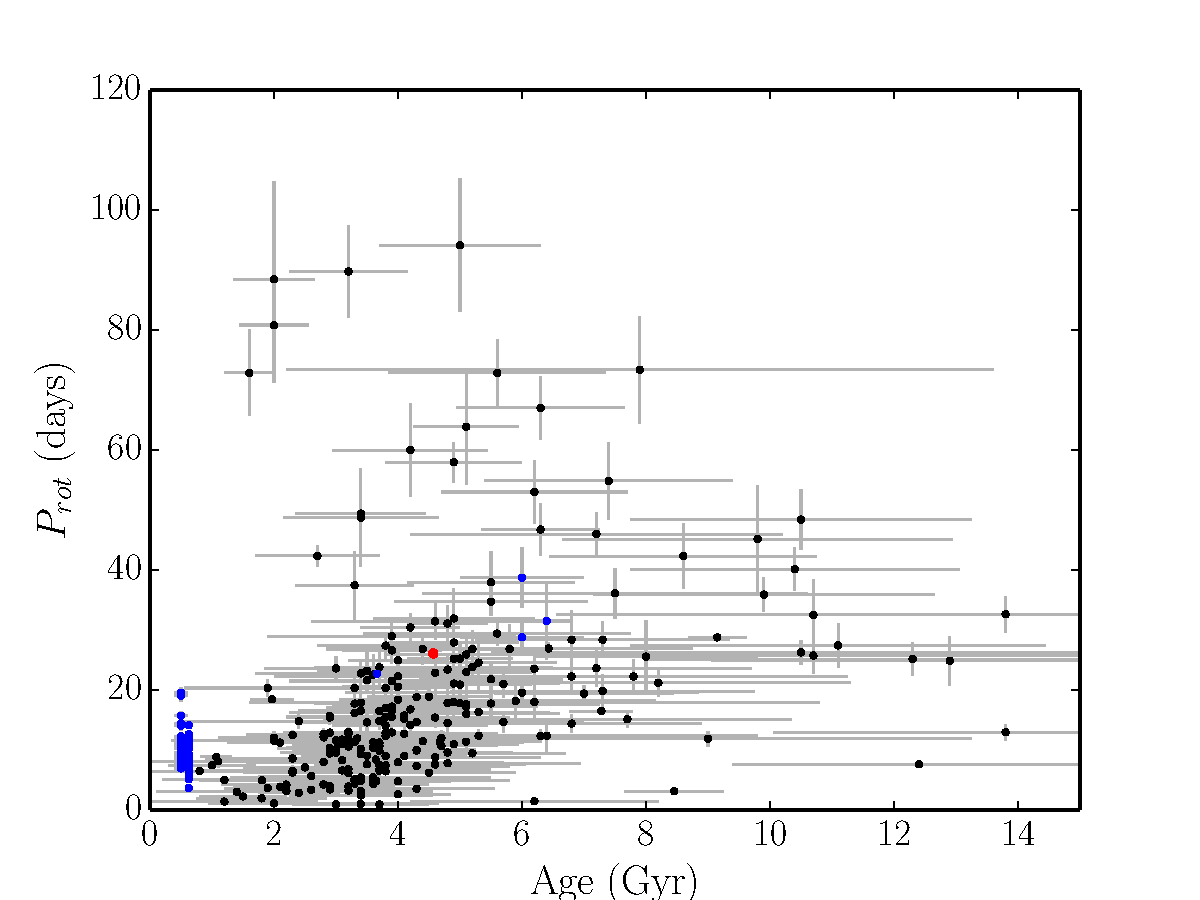
\includegraphics[width=6in, clip=true, trim=0 0 0.5in 0]{p_vs_a_paper2.pdf}
\caption{Photometric rotation period vs age for \nastero$~$ {\it Kepler}
	targets (black) plus cluster and field stars (blue). The Sun is shown
	in red.
\label{fig:p_vs_a}}
\end{center}
\end{figure}

\begin{figure}[ht]
\begin{center}
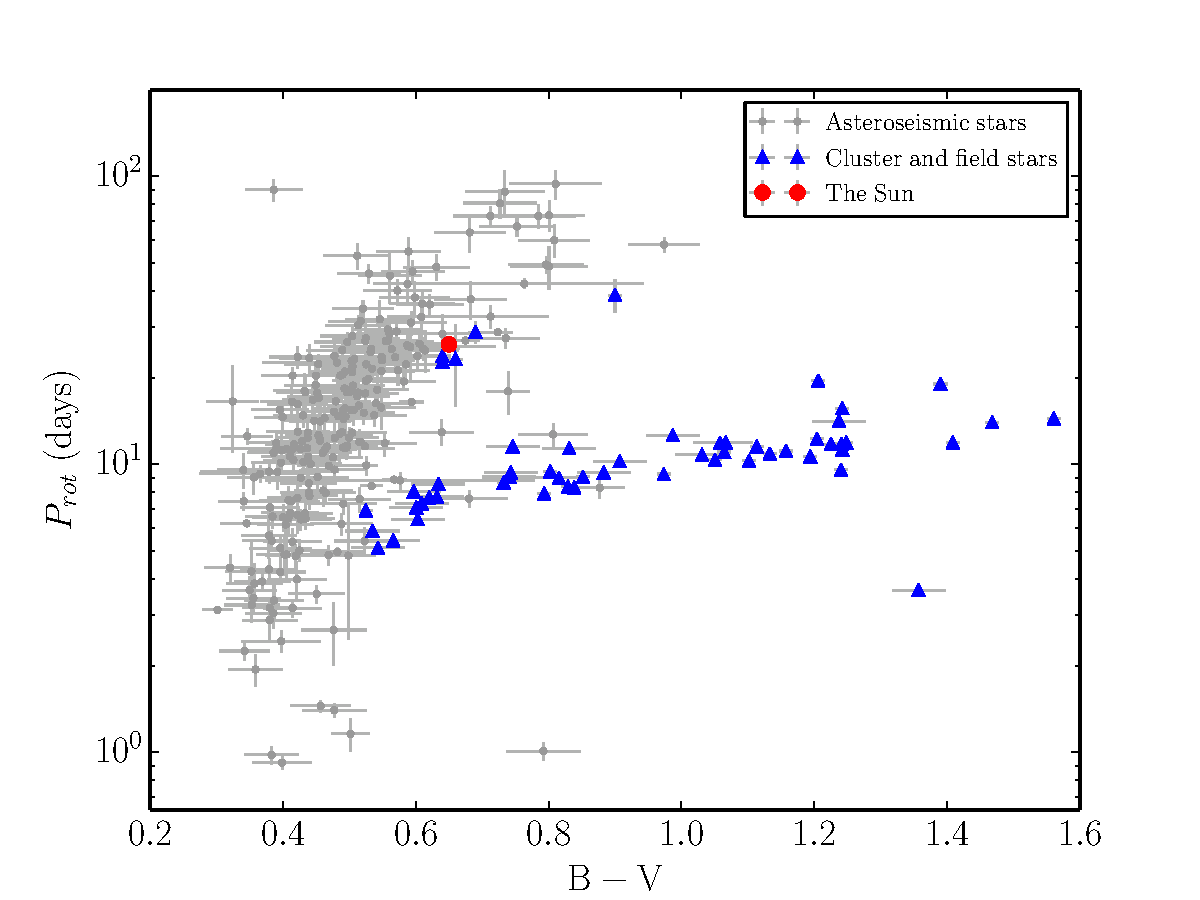
\includegraphics[width=6in, clip=true, trim=0 0 0.5in 0]{p_vs_bv_paper2.pdf}
\caption{Photometric rotation period vs $B-V$ colour for the data described in
	figure \ref{fig:p_vs_a}.
\label{fig:3d}}
\end{center}
\end{figure}

\begin{figure}[ht]
\begin{center}
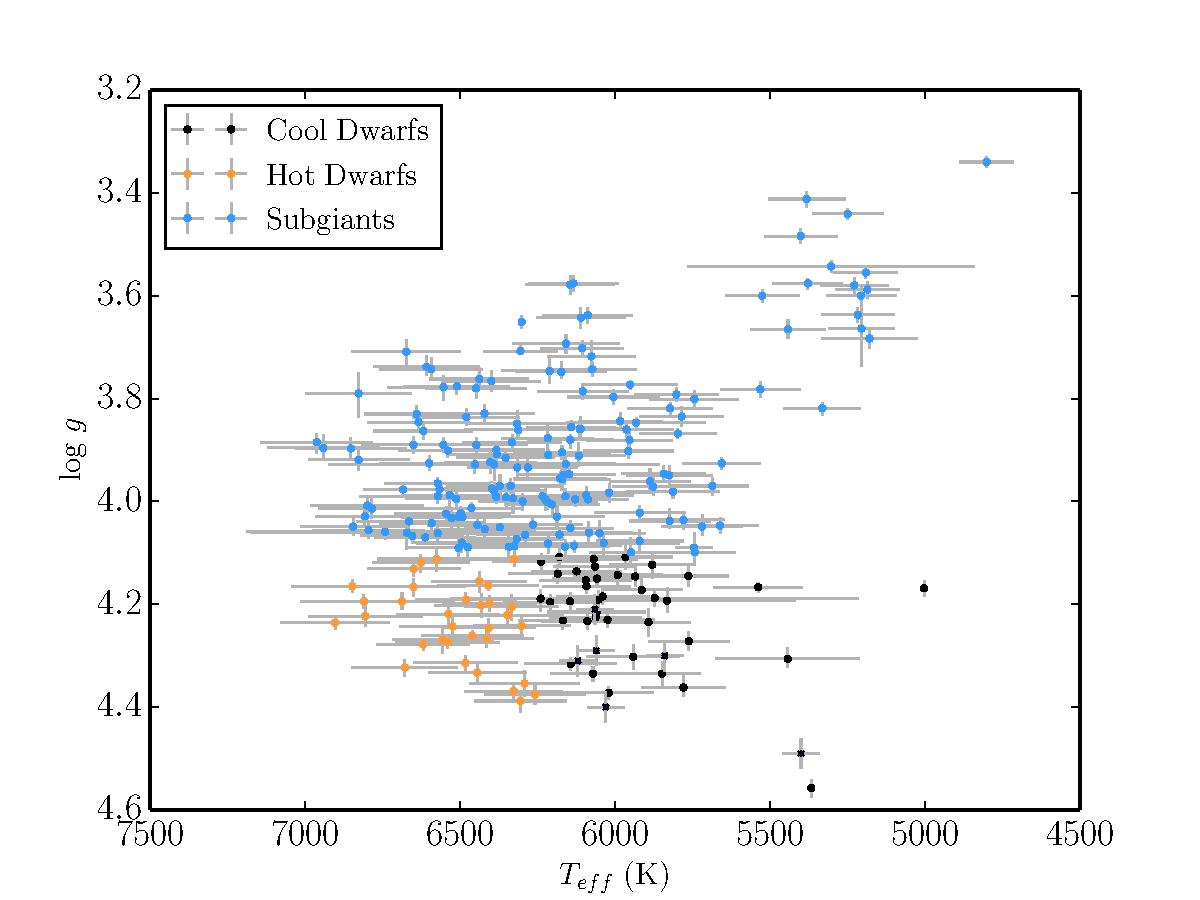
\includegraphics[width=6in, clip=true, trim=0 0 0.5in 0]{logg_vs_t_paper.pdf}
\caption{\logg$~$vs \teff$~$for the \nastero$~$asteroseismic stars. Hot dwarfs
with \teff$~>$ 6250 K and \logg$~>$ \subcut are red, subgiants with \logg$~<$
\subcut are blue. Only the black cool dwarfs with \teff$~<$ 6250 K and
\logg$~<$ \subcut are expected to follow the gyrochronology relation in
equation \ref{eq:Barnes2007_2}.
\label{fig:logg_vs_t}}
\end{center}
\end{figure}

\begin{figure}[ht]
\begin{center}
	\subfigure[Coma Berenices and field stars.]{
            \label{fig:CF45}
	    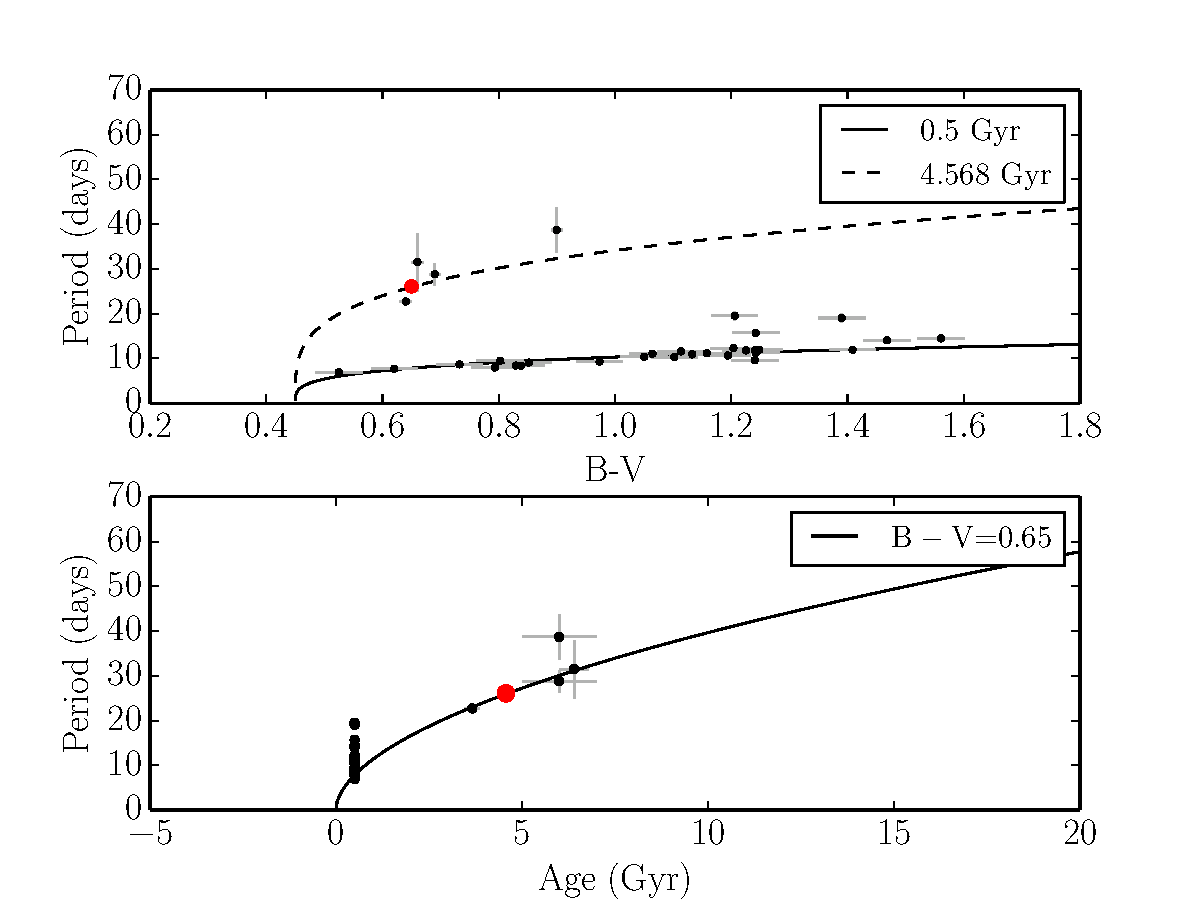
\includegraphics[width=4in, clip=true, trim=0 0 0.5in 0]{showCF45.pdf}
        }
	\subfigure[Hyades and field stars.]{
            \label{fig:HF45}
	    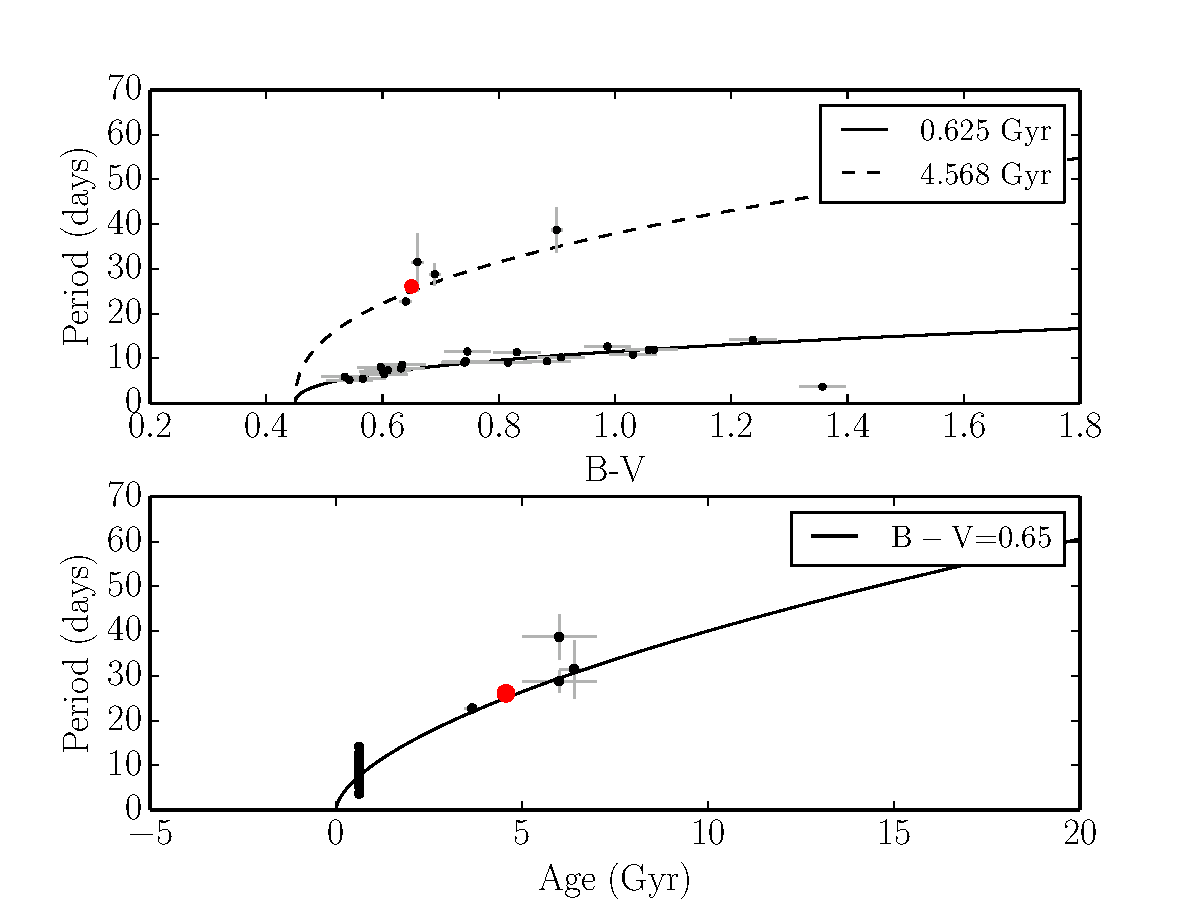
\includegraphics[width=4in, clip=true, trim=0 0 0.5in 0]{showHF45.pdf}
        }
    \end{center}
    \caption{ Individual fits to the clusters and field stars. The Sun is the
	    red point. Top panels show period vs $B-V$ with Solar and cluster
	    age isochrones. Bottom panels show period vs age with the period-
	    age relation for a constant $B-V$ value of 0.65 (Solar $B-V$).
\label{fig:subfigures1}}
\end{figure}

\begin{figure}[ht]
\begin{center}
	\subfigure[0.5 Gyr (age of the Coma Ber)]{
            \label{fig:5}
	    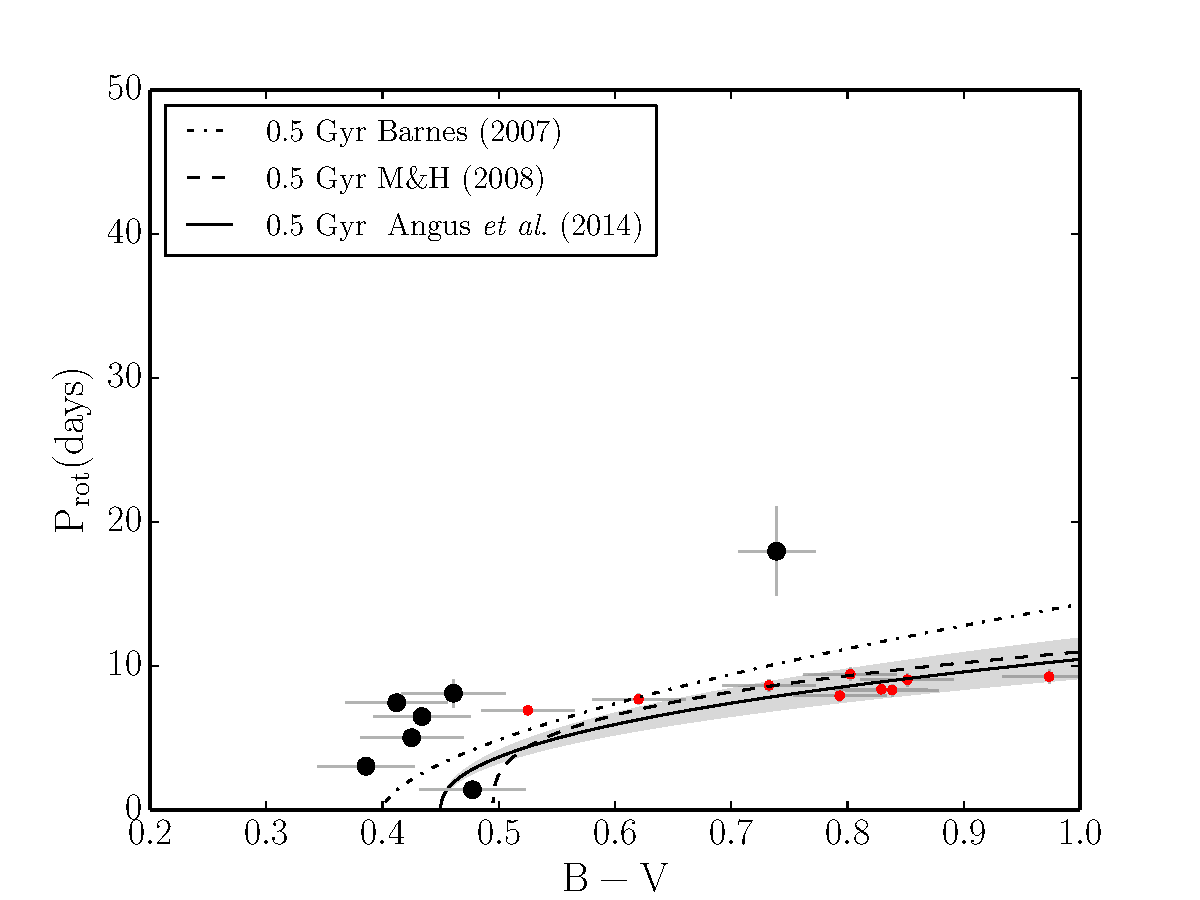
\includegraphics[width=3in, clip=true, trim=0 0 0.5in 0]{p_vs_bv0.pdf}
        }
	\subfigure[0.625 Gyr (age of the Hyades)]{
            \label{fig:625}
	    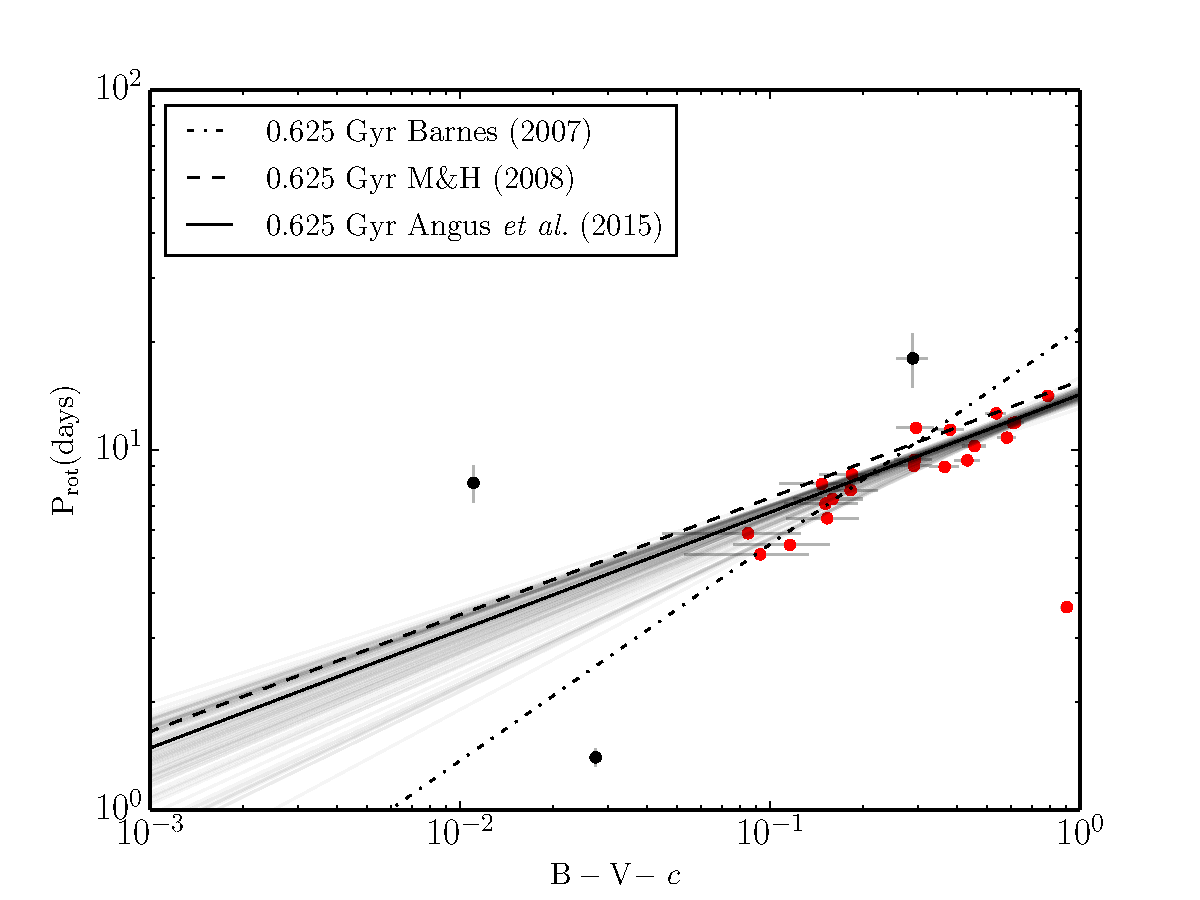
\includegraphics[width=3in, clip=true, trim=0 0 0.5in 0]{p_vs_bv1.pdf}
        }
	\subfigure[2 Gyr]{
            \label{fig:2gyr}
	    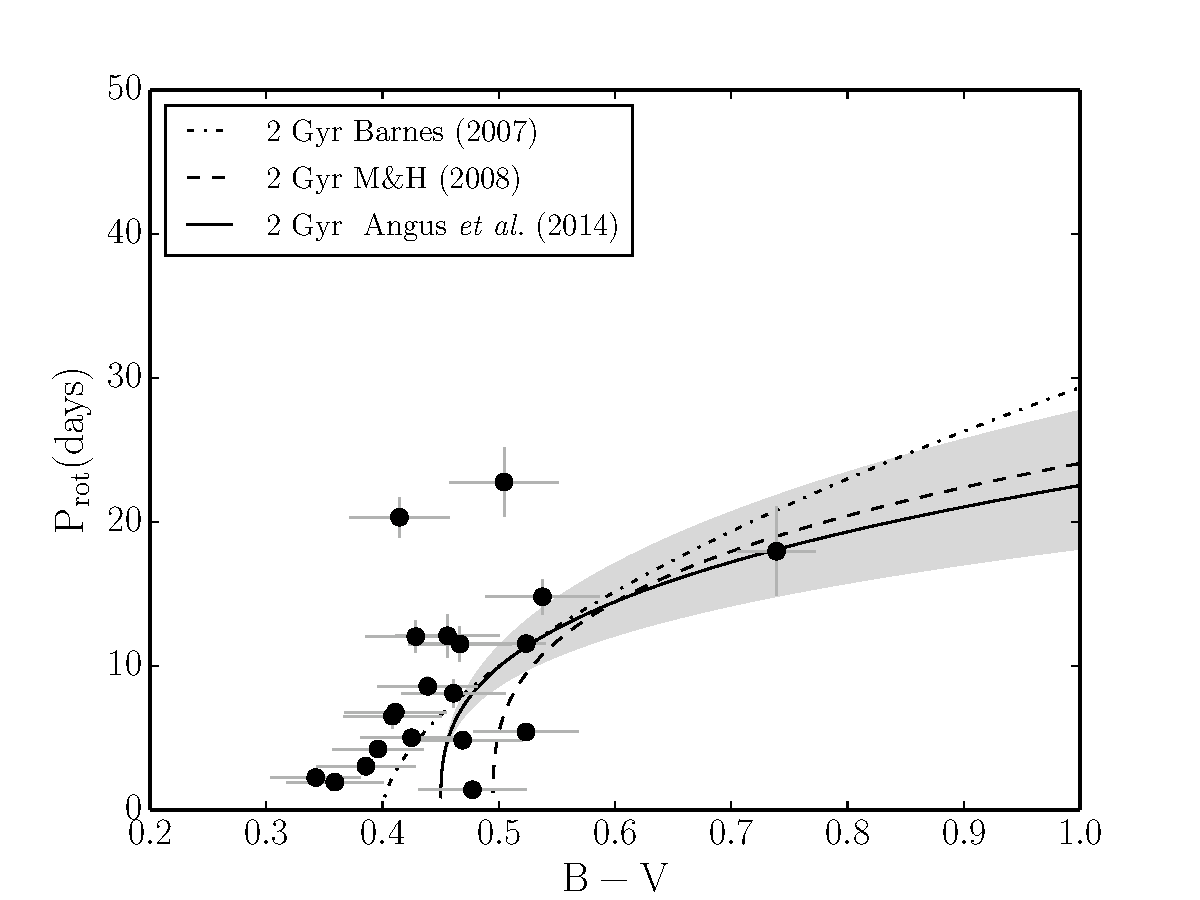
\includegraphics[width=3in, clip=true, trim=0 0 0.5in 0]{p_vs_bv2.pdf}
        }
	\subfigure[5 Gyr]{
            \label{fig:sungyr}
	    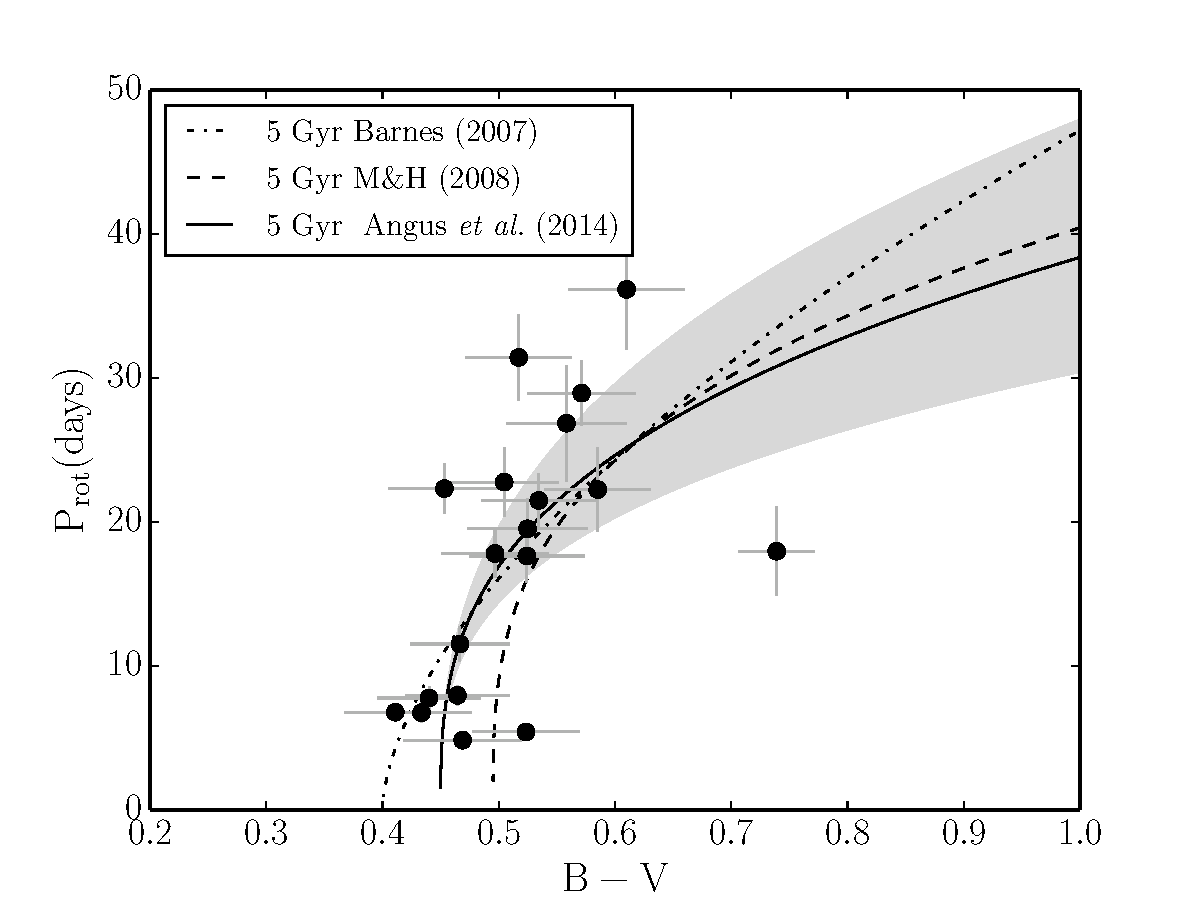
\includegraphics[width=3in, clip=true, trim=0 0 0.5in 0]{p_vs_bv3.pdf}
        }
	\subfigure[8 Gyr]{
            \label{fig:8gyr}
	    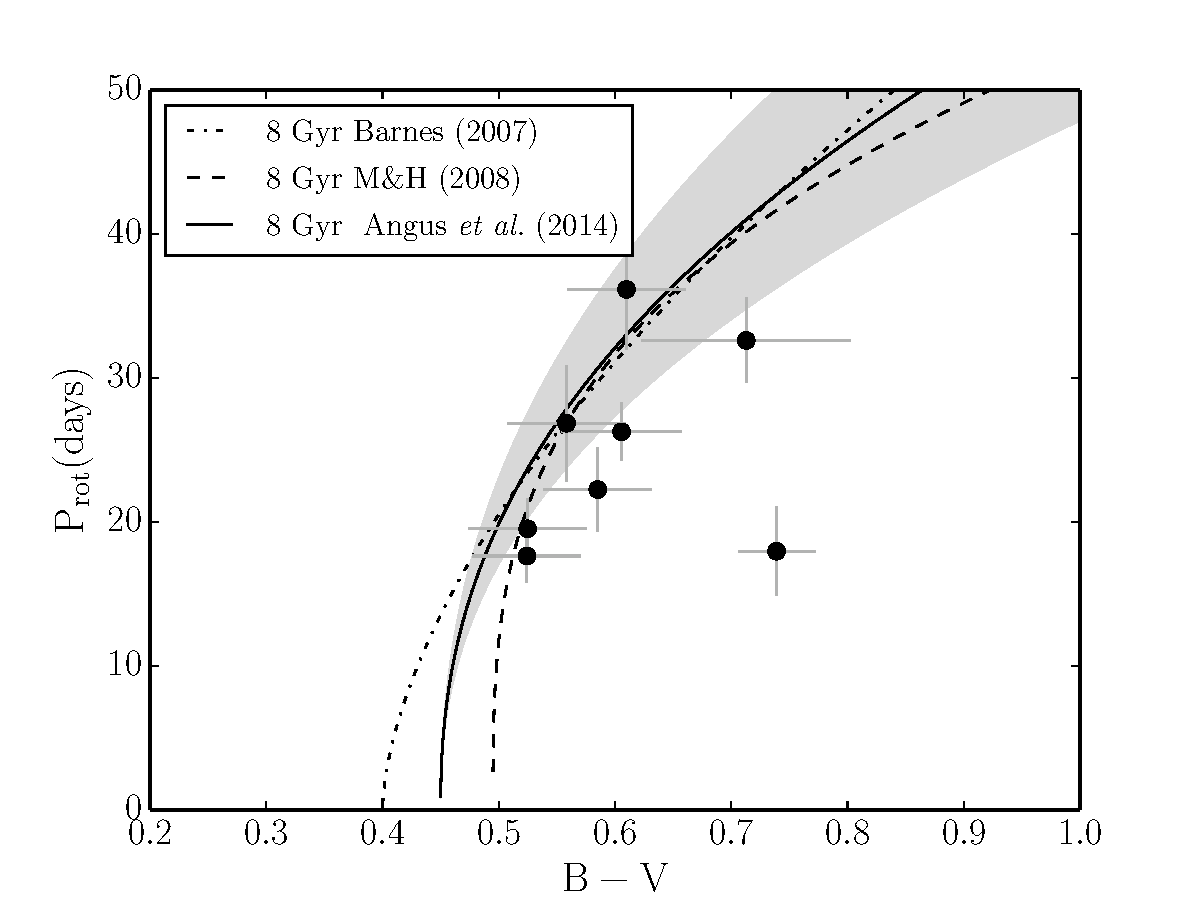
\includegraphics[width=3in, clip=true, trim=0 0 0.5in 0]{p_vs_bv4.pdf}
        }
    \end{center}
    \caption{ \prot vs $B-V$ colour for dwarfs within 1$\sigma$ of the reference age with the new gyrochronology relation and \citet{Barnes2007}, and \citet{Mamajek2008} for comparison. Asteroseismic targets are black and cluster and field stars are red. The shaded regions represent the 16th and 84th percentile uncertainties.
   \label{fig:subfigures2}}
\end{figure}

% \begin{figure}[ht]
% \begin{center}
% 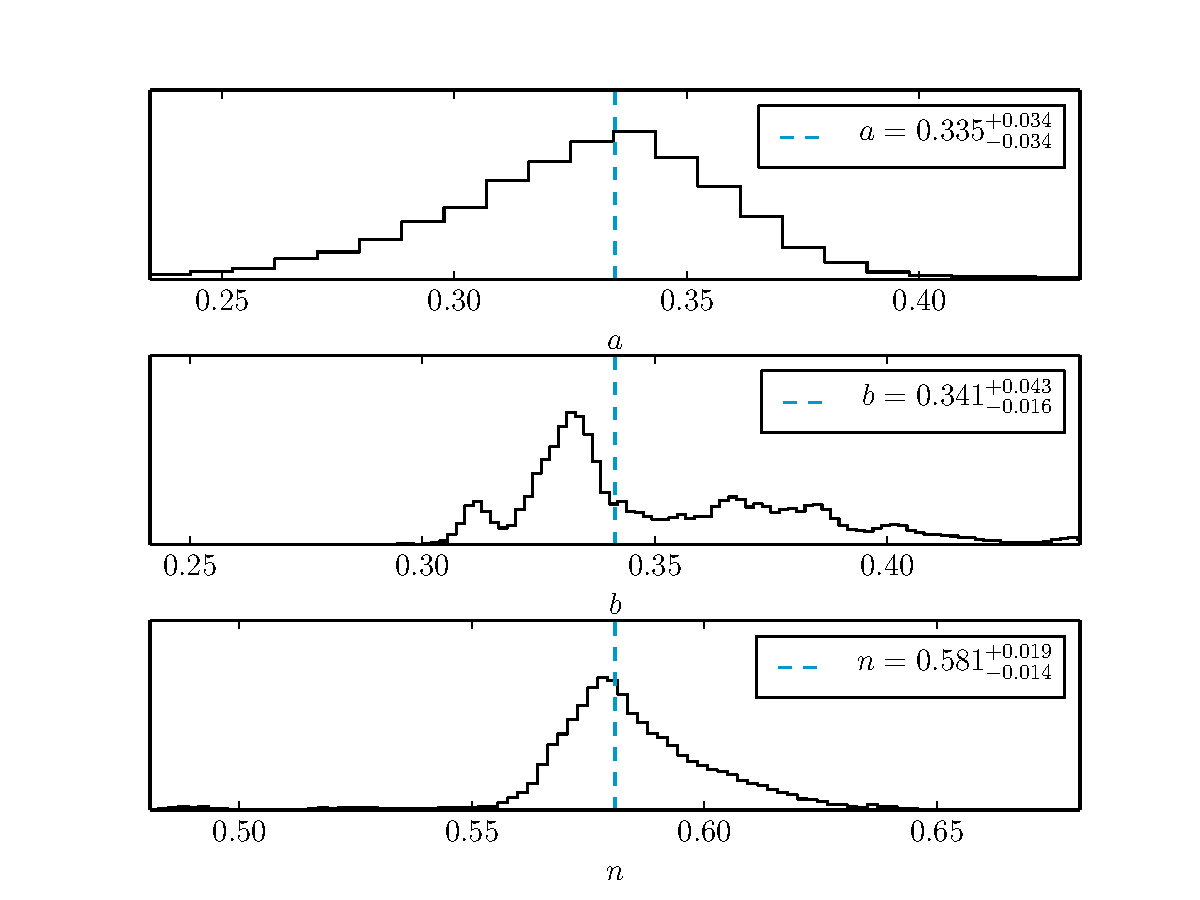
\includegraphics[width=6in, clip=true, trim=0 0 0.5in 0]{marg_posteriors.pdf}
% \caption{Marginalised posterior PDFs of the three gyrochronology parameters; $a$, $b$ and $n$, conditioned on the asteroseismic stars, the field stars, the Hyades and Coma Berenices.
% \label{fig:marg_posteriors}}
% \end{center}
% \end{figure}

\begin{figure}[ht]
\begin{center}
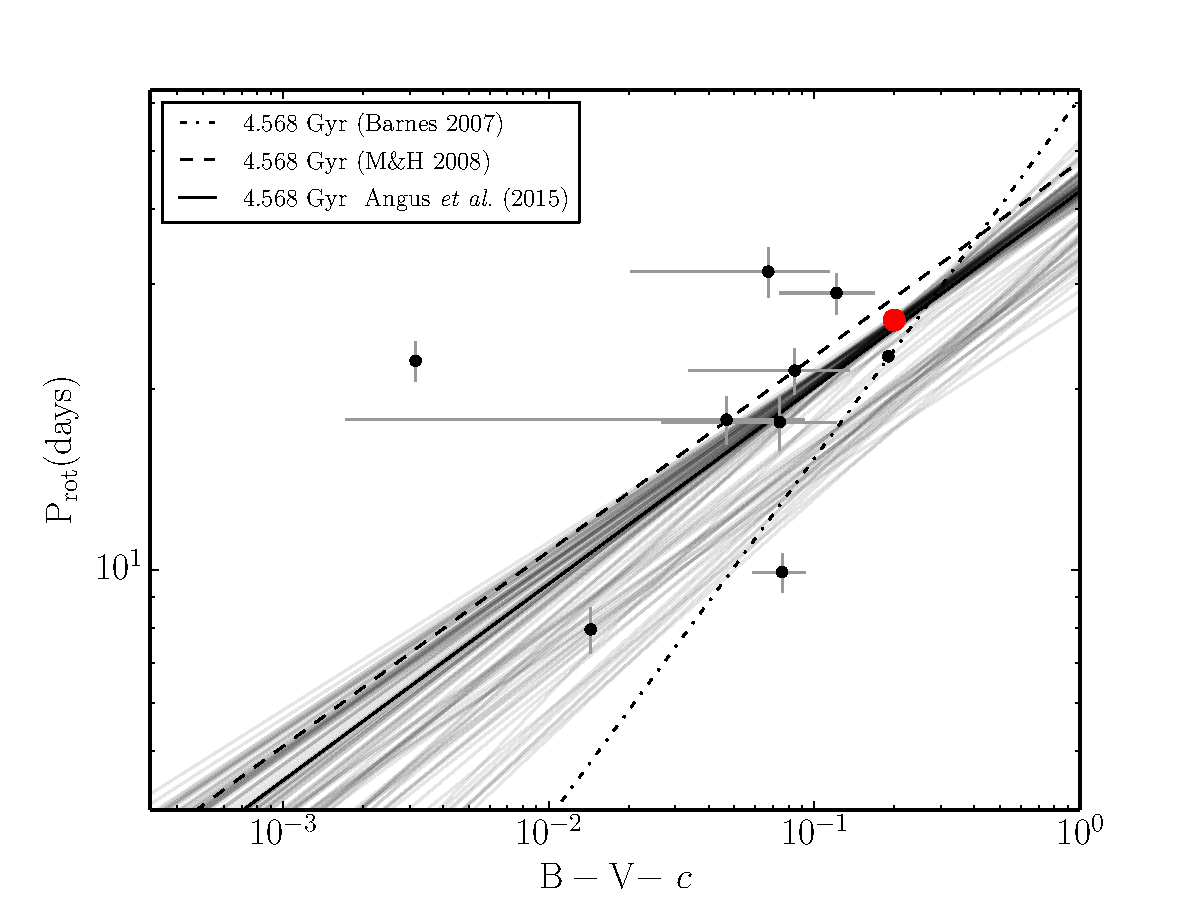
\includegraphics[width=6in, clip=true, trim=0 0 0.5in 0]{p_vs_bv_solar.pdf}
\caption{Rotation period vs $B-V$ colour for dwarfs with age within 1$\sigma$ of the Sun's age, 4.568 Gyr. The Sun is the red point.
\label{fig:p_vs_bv_solar}}
\end{center}
\end{figure}

\begin{figure}[ht]
\begin{center}
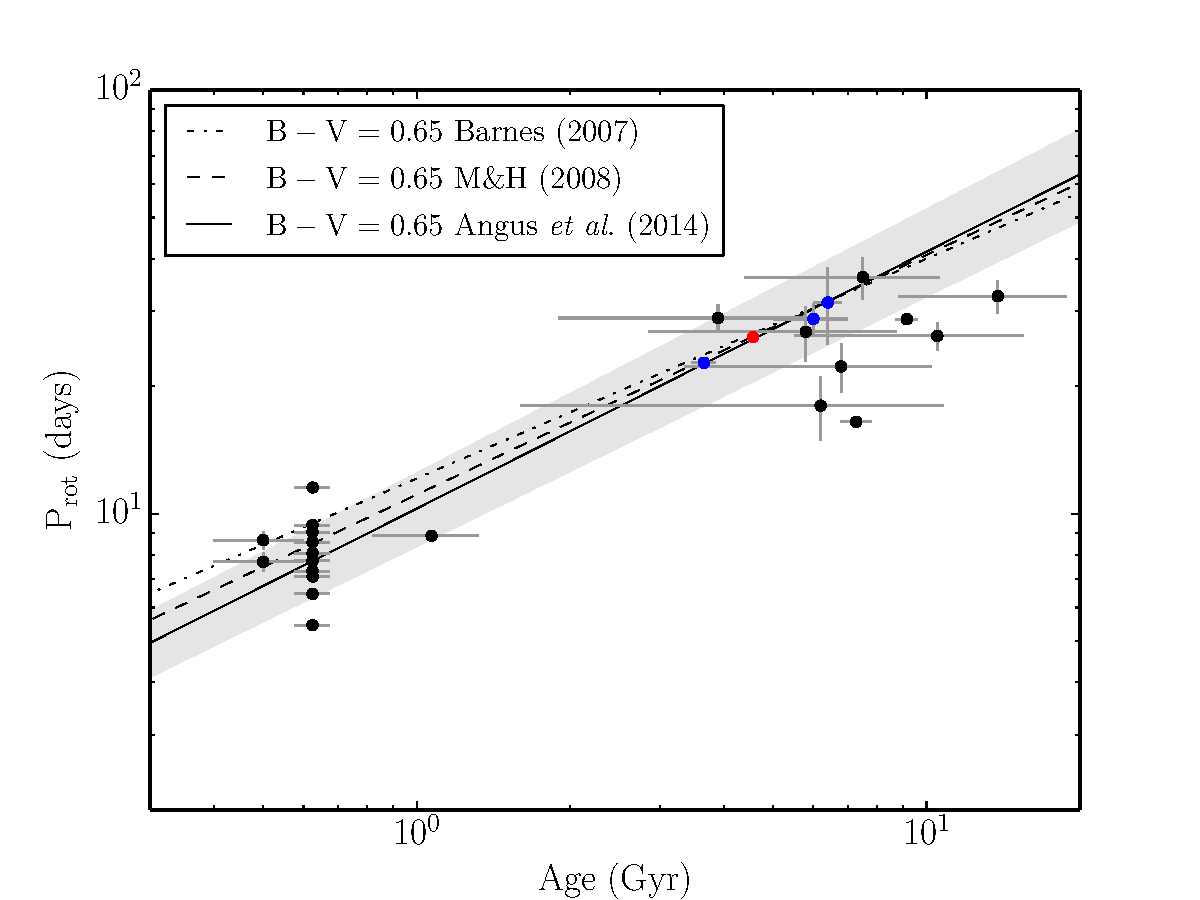
\includegraphics[width=6in, clip=true, trim=0 0 0.5in 0]{p_vs_a_solar.pdf}
\caption{Rotation period vs age for cool dwarfs with colour within 10\% of the
	Sun's: 0.65, with gyrochronology relations of \citet{Barnes2007},
	\citet{Mamajek2008} and this work. The shaded region represents the
	16th and 84th percentile uncertainties. The Sun is shown in red and the
	field stars, $\alpha$ Cen A, 18 Sco and 16 Cyg from left to right, are
	shown in blue.
\label{fig:p_vs_a_solar}}
\end{center}
\end{figure}

\begin{figure}[ht]
\begin{center}
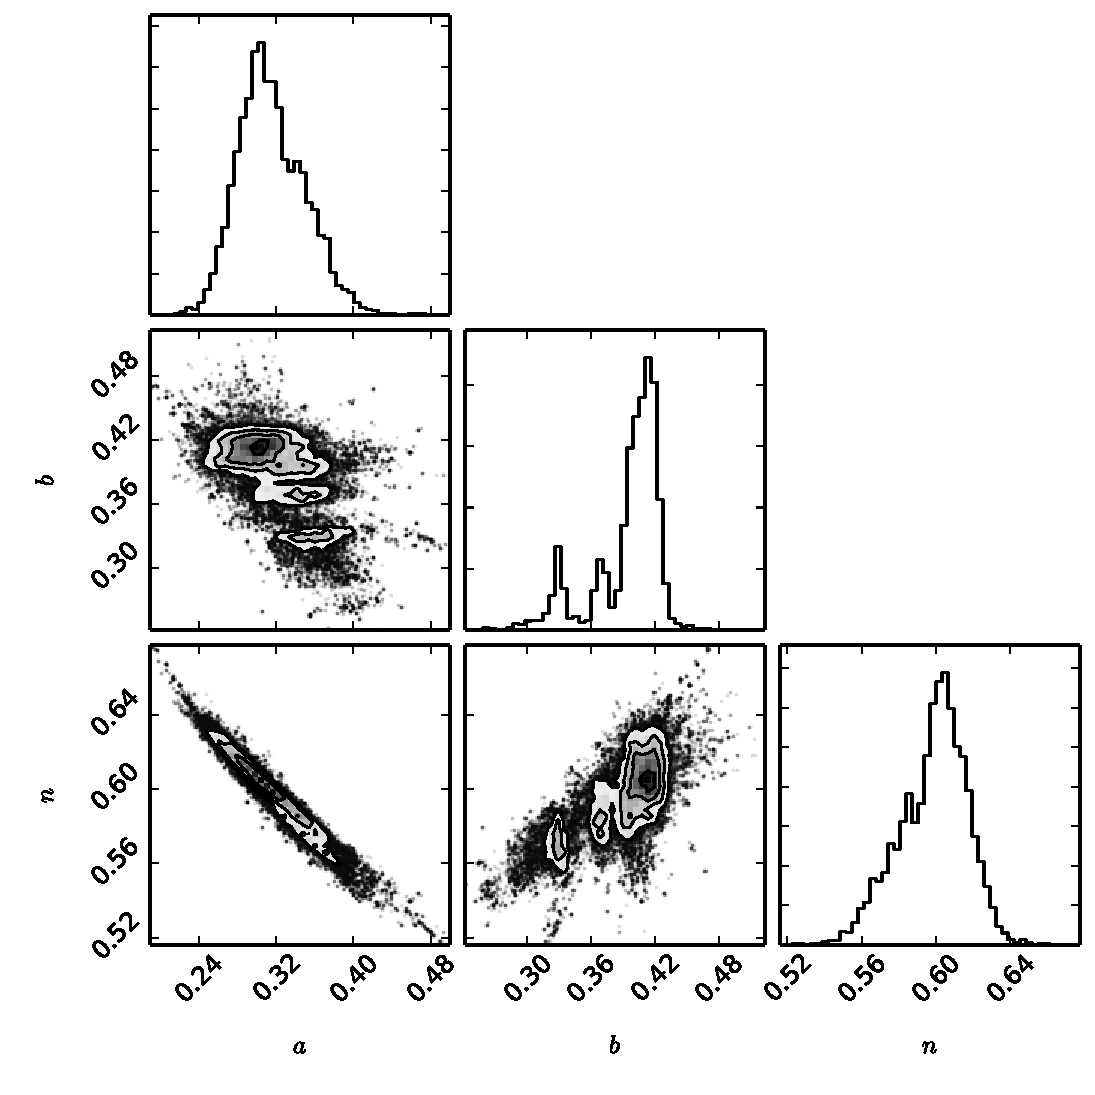
\includegraphics[width=6in, clip=false, trim=0 0 0.5in 0]{small_triangleACHF45.pdf}
\caption{Marginalised likelihoods for the three gyrochronology
parameters, $a$, $b$ and $n$. All three parameters are correlated and $b$ is
slightly multi-modal. This plot was made using triangle.py
\citep{Foreman-Mackey_triangle}.
\label{fig:triangle}}
\end{center}
\end{figure}

\end{document}
